% prevent footnotes from running onto multiple pages.
\interfootnotelinepenalty=10000

\section{Introduction}

\todo{DELETE ALL TODOs}

\todo{SPELLCHECK - including abstract!!}

\todo{This paragraph uses the work ``held'' with CIP}

\todo{!!!!! - recheck abstract}

\todo{!!!!! - spacing}

% Questions to Saroj, with answers
%
% Space everywhere.
% pg 4 - what does this mean?
%    --- don't claim 60bp is the hard line for "yes/no" .... hedge more

% pg 23 - was the Cochraine sentence too informal?
% pg 26 - does this means move table here?
% pg 67 - Saroj wanted multi-line paragraphs indented?
%    --- he saw it as one paragraph with equations in it.  The non-indented lines were new paragraph
% pg 71 - clustered error
%    - did not ask
% pg 83 - what does this mean?
%    - spacing.  "try fonts", "try resizing"
%    -  "looks unprofessional with so much space"
% pg 93 - what does this mean?
%   "be balanced"
%   "same order of magnitude"




Covered interest parity (CIP) is a no-arbitrage condition relating the prices of international bonds, currencies, and currency forwards.  Before the Global Financial Crisis of 2007-2008 (henceforth ``the crisis''), the CIP relationship held.  That is, from January 2000 to May 2008, the yield from the arbitrage trade (without leverage) using interest rate swaps was under 30bp.  After the crisis, the relationship has not held.  From November 2009 to March 2017 (the last date studied), the yield from the arbitrage trade (without leverage) has exceeded 60bp, which is more than the value at which banks, even ones restricted by post-crisis legislation, should trade it.  (See Figure~\ref{max_CIP_basis_spread_swap}.)  The research community does not understand why banks are not performing this arbitrage trade, which has a high guaranteed return.  This thesis examines the problem, using rates from long-term corporate bonds.


\begin{figure}[h]  % h = here
\textbf{\caption{\label{max_CIP_basis_spread_swap} Max CIP basis spread for 5-year horizon}}
\includegraphics[height=3.1in]{images/BasisSpread_all_swap_5Y}
Note: {\small Maximum CIP basis spread, calculated with a 5-year swap rates.  The max CIP basis spread is the return an arbitrageur would get when trading without leverage.  Here, it is calculated over the 10 currencies studied: USD, EUR, JPY, CHF, GBP, AUD, CAD, SEK, NOK, and NZD.}
\newline Source: Bloomberg L.P.
\end{figure}



\todo{footnote explaining interest rate swaps are the ``Bond'', and saying ``swap rate'' is the rate of the interest rate swap.}

%Covered interest parity stopped holding true in 2008.  The condition has been described as ``a bedrock''\cite{Coffey2009} and ``the closest thing to a physical law in international finance''\cite{Borio2016}, but it stopped working and has yet to reassert itself.  
%Covered interest parity relates government bond markets, which trade over 500B USD daily, to the currency markets, which do roughly 2.3B USD (equivalent) daily in spot and forwards.

% currency markets do 1.6B USD (equivalent) in spot and 0.7B USD (equivalent) in forwards daily.  

%``perhaps the best established principle in international finance''\cite{Avdjiev2016}
% ``the closest thing to a physical law in international finance''\cite{Borio2016}
% ``a bedrock of international economics''\cite{Coffey2009}

% define CIP

Covered interest parity is best explained by example.  Starting with 1M USD, you could invest it in a 5-year U.S. Treasury bond and get a return of 1.7\%.  Alternatively, you could convert that 1M USD into 0.9M EUR and buy two things: a 5-year German bund with a return of -0.41\%, and a forward contract that locks in the price today of exchanging the EUR back into USD in 5 years.  Investing either of those ways --- directly in U.S. Treasury bonds or via EUR in Germany bund --- should give the same overall return (assuming both governments are considered equally sound).  That condition is called ``covered interest parity''.

\todo{In the following figure description, the word ``median'' can be replaced by ``spent more than half its time''}


% History of CIP and CIP deviations

%Before the Global Financial Crisis of 2007-2008 (henceforth ``the crisis''), CIP held.  That is, most of the time the returns between major currencies differed by less than 28 basis points.  (See Figure~\ref{CIP_basis_govt}.)  Since the crisis, it has grown and sometimes reaches over 1\% (or 100bp).  These deviations have persisted long after the crisis, which is curious because the academic community had assumed any deviations could be easily arbitraged away.  The markets are deep and, using government bonds, the trade is risk-free and has an infinite Sharpe ratio.

% Note, pre2007 number for swaps is 6 basis points

% After all, foreign exchange does 1.6B USD (equivalent) daily in the spot market and 0.7B USD (equivalent) daily in the forward market.\cite{BIS2016}

% Previous work

The deviations from CIP were identified soon after the crisis.  Some researchers ascribed it to counterparty risk and banks requiring more capital.\cite{Coffey2009}  But the deviations persisted, even after banks had recapitalized.  Researchers have started identifying patterns and hypothesizing on both the cause of the deviations and why prices have not returned to CIP.  Causes for the deviation include central bank policy\cite{Du2017}, regulatory changes\cite{Liao2016}, and hedging demand\cite{Borio2016}.  More puzzling has been why prices do not return to CIP.  A common explanation has been new banking regulations enacted after the crisis: the Dodd-Frank Act and Basel III Accord lessen the amount of leverage that banks can use.\cite{Du2017,Liao2016,Borio2016}  Recently, a paper\cite{Rime2017} has suggested that it is because few banks have a good enough credit rating to perform the arbitrage and a news article\cite{Duffie2017} has suggested debt overhang induces banks away from guaranteed trades like arbitrage.

\todo{Don't like ``allow better measurement'' in the following paragraph}

CIP has been studied using interest rates from various securities, both short-term and long-term.  This thesis's work focuses on long-term corporate bonds, where the firm has issued bonds in multiple currencies.  If a firm issued a bond in multiple currencies, those bonds have nearly identical risk, unlike government bonds or swap rates, where the risks differ.  If other differences in the corporate bonds (such as maturity) can be accounted for, long-term corporate bonds allow for better measurement of CIP.

The major existing work covering corporate bond rates and CIP was done by Liao\cite{Liao2016}.  He focused on firms issuing bonds in foreign currencies to get a lower interest rate.  He found that firms issued more foreign bonds when overseas interest rates were lower.  He defined the ``residualized credit spread differential'' as a function of corporate bond rates and swap rates, and then showed that this measure was correlated with CIP deviations, when calculated using the swap rate.  

\todo{Can I make ``price of a swap'' clearer in the next \P?}

Liao's study used swap rates instead of government bond rates for the reference rates measuring CIP deviation.  This is common in the field\cite{Du2017,Borio2016,Avdjiev2016}.  However, swap rates depend on interbank loan indices, like LIBOR, and bank default risks are not identical across currencies, nor stable during a financial crisis.  Moreover, swap rates are the price of a variable contract, not of a bond, and bonds are necessary for measuring CIP.

%\todo{ include something like: ``Since most other papers in the field of CIP use the swap rate for long-term interest rates, this thesis may have a unique contribution.''}

% Use of long-term swaps
%Avdjiev2016, page 2, Figure 1, ``cross currency basis swap spreads''
%Borio2016, page 50, Box B, ``interest rate swap rate''
%Coffey2009 --- NO PROBLEM ---used 3 month graphs with LIBOR or TBill
%Du2017, --- Page 11, "cross currency basis swap" (floating rate EUR for floating rate USD + fixed).  PROBLEM IS MITIGATED BY ALSO USING  Bund, but also uses "tenor basis swap", which swaps 3M LIBOR for 1M LIBOR + fixed basis payment.  
%Rime2017,  --- NO PROBLEM --- short time only

% The first finding in this thesis is that the swap rate, while talked about in the press\cite{FT_swap, TheEconomist} and academic circles\cite{Jermann2017} as an interest rate, is not an interest rate.  That is, the market contains bonds of equivalent risk and duration with a better rate.  I hypothesize --- but do not test --- that companies called ``structured investment vehicles'' (SIVs) made the swap rate act like an interest rate up until they stopped operation, during the crisis.  A number of papers in the field of CIP use the swap rate for long-term interest rates and their results should now be examined with a critical eye.

% Liao's study that CIP-LOOP held was based on a regression of bonds where the firms had issued in more than one currency.  If that regression fully described the international bond market, you would expect the same results (within error) from a regression of firms that issued in only one currency.  That regression is significantly different.  I hypothesize that when a firm issues a bond in a foreign currency, that bond is not priced by local traders, but by the home country's traders.  This implies that CIP-LOOP holds for bonds relative to the bonds from its home country, but not to bonds from a different home country.  


In this thesis, I reproduce Liao's work with swap rates and then reevaluate it using government bond rates.  The results are better (correlations are higher) with government bond rates.  I then estimate the CIP deviation using long-term corporate bonds.  My results show that, since November 2011, CIP deviations, when calculated using corporate bonds, are lower than when measured with swap rates or government rates.  During that period, the median deviation is 48bp, which is the correct scale for the threshold where banks perform the arbitrage trade.  I conclude that the CIP deviations measured with corporate bonds fulfill our expectations on how CIP deviations should behave and that they should be preferred to CIP deviations measured with swap rates and government rates.

\todo{!!!!! Saroj had comment on 51bp.  ??? ``This result are very preliminary, so better with explain you got < 60bp}
\todo{!X Check November 2011 from above in the data.}


\todo{ Insert graph or figure with something I found.}

% The final finding is that CIP does not have to hold under uncertainty.  I demonstrate this with a simple two-period model where the two interest rates (e.g., USD and EUR) in the second period are not determined at the start.  For CIP to hold, an equation containing the second period's interest rates would have to be separable, which is not the case in general.  Nor does it seem likely when the interest rates are normally distributed.  I suggest that models based on options pricing, such as \cite{Black1995}, should be considered for CIP research in the future.


\subsection{Literature Review}

\todo{Make sure this all uses the past tense}

There is a long history associated with covered interest parity.  Discussion of CIP even predates the creation of the first currency futures in 1970.\cite{Kolb2010}  This subsection will focus on work done after the crisis and concentrate on those that study long-term bonds.  

% % futures in 1970 at International Commercial Exchange in New York.  No need - Brenton Woods.  CME in 1972 

Shortly after the crisis, CIP deviations were identified and studied.  The causes were believed to be transitory: counterparty risk and banks requiring more capital.\cite{Coffey2009}  As the deviations persisted, researchers have started identifying patterns and hypothesizing on both the cause of the deviations and why prices do not return to CIP. 

% This is Sushko
Borio et al.\cite{Borio2016} and Sushko et al.\cite{Sushko2016} focused on the foreign exchange (FX) forward market, which trades less volume than the FX spot and bond markets.  They looked at a few causes of deviations in that market: cross-border funding by firms (who borrow in foreign currencies and then hedge the liability) and institutional investors' strategic hedging.  

Their explanation for why deviations persist was that banks perceive risk as being higher than before the crisis.  Counterparty risk, as proxied by the OIS-LIBOR spread, was higher.  Collateral risk, measured by FX options, was also higher.   When collateral risk is higher, REPO becomes more expensive and the arbitrage trade to close the CIP deviations is less scalable and less profitable.  Other factors included central banks buying bonds, which also drives up REPO rates, and new regulations, which put an upper bound on the leverage banks can obtain.  

% Borio pg 60-61
% Their study did show that with longer term bonds (2-year bonds vs. 3-month bills), the effect of counterparty risk and collateral risk was much smaller than the effect from the demand for FX forwards.
% The counterparty risks had a strong effect on CIP basis measured with 3-month deposits, but only a smaller effect on CIP basis with 2-year bonds, which were mostly subject to the demand of FX forwards.


%Borio's Since 2014, attention has shifted to other factors and constraints. Most studies have invoked some notion of capital constraints of CIP arbitrageurs in the face of FX swap funding demand from banks (Iida et al (2016)), from foreign currency bond issuers (Liao (2016)) or from broader saving and investment imbalances (Du et al (2016)).4 Similarly, Shin (2016) attributes the persistent deviations from the CIP to a systemic risk factor linked to the US dollar’s role as the global funding currency.5

%- balance sheet
%- pricing of risk (counter party and collateral)
%- OIS-LIBOR spreads
%- REPO availability ``scalability constraint''

% Borio
% balance sheet capacity
%And even if risks were lower, new regulation limits the amount of leverage banks are allowed. 
% measure hedging demand by looking at bank balance sheets, flows. 
% Fed, Bank of Japan buy up bonds, driving up REPO prices
% two-year bond shows little pushback - just FX hedging effect

 
Du et al.\cite{Du2017} presumed that CIP deviations were caused by persistent imbalances in investment demand and focused on why CIP did not reassert itself.  They found significant CIP deviations even when they restricted themselves to looking at bonds in multiple currencies from Kreditanstalt f\"ur Wiederaufbau (KfW), a development bank owned by the federal and state governments of German.  These bonds are liquid and safe (backed by the German government) and the authors concluded that arbitrage was not limited by transaction costs nor credit risk.

Du et al.\ used the OIS-LIBOR spread as a proxy for balance-sheet costs and found that it explained at least half of short-term CIP deviations.  In the same vein, they found correlations between the CIP deviations and other trades that involve liquidity risk, such as the swap of LIBOR 1M for LIBOR 3M, known as the ``tenor''.  Du et al.\ discovered an interesting effect that CIP deviations increase dramatically when the forward contract was not settled before the quarter ends.  They believe this was a novel limit to arbitrage where European banks, who have to report their holding at the end of the quarter, were trying to profit from arbitrage only when it would not appear publicly in their books.  

%Sushko's  Du, Tepper, and Verdelhan (2016) formally establish the CIP arbitrage opportunities that cannot be explained away by credit risk or transaction costs.

% INCLUDE? : higher interest securities usually have higher CIP basis

% % Du:

% %4 findings:
% %CIP increase at quarter's end
% %balance sheets account for 1/2 of spread  (estimated by OIS - LIBOR spread)
% %High-interest rate currencies have positive basis, low have negative
% %cross-currency basis related to 3-month/1-month tenor basis

% %2 causes
% %increased cost of financial intermediation post-crisis and persistent international imbalances in investment demand %and funding supply across currencies.

% A paper by Du et al.\cite{Du2017} studied CIP at short and long durations.  One of their findings was that CIP basis increased for short-terms at the end of the quarter.  Liquidity may be tighter at the end of the quarter, but the authors note that European banks must also report their balance sheets to investors.  If bank owners want to hide their exposure to currencies, they must unwind their positions before they have to be reported.  This effect was one of the reasons Du et al.\ believed that the increased cost of financial intermediation was a limit to arbitrage for CIP.

% Du et al.\ believe balance sheet costs were another limit to arbitrage.  They estimated the cost of leverage from the relationship of the overnight rate (OIS) to the LIBOR rate and the interest on excess reserves (IOER).  Give the large spread between these, a bank that can borrow at the OIS rate and make a profit in either LIBOR or IOER.  Thus, any arbitrage of covered interest parity must make a return larger than that spread.  They documented this for the arbitrage between the German bund and KfW bonds, which are also guaranteed by the Federal Republic of Germany.  Du et al.\ estimate that a third to a half the CIP basis is due to this spread.

% Du et al.'s third finding was that countries with a high interest rate had a positive CIP basis and those with low interest rates tended to have a negative CIP basis.  This correlation was done with 5-year swaps as well as 5-year U.S. Treasury rates.  Their last finding was that the cross-currency basis (the difference between two countries swap rates) is correlated with the tenor basis, the spread between one-month and 3 month LIBOR.  

% Du et al.'s did look at two things specific to the long-term CIP basis.  They plotting the 5-year CIP basis using swap rates.  They also computed the value at risk (VaR) for a trade using the 5-year swap.  In 2009, the VaR was over 20\%, which may have discouraged the trade in following years.  Beyond these, most of their results were with short-term CIP basis or might apply to either.  Du et al.\ did most of their studies with LIBOR and swaps, but some involve government rates such as IOER, U.S. Treasury bonds and German bond rates.

% Avdjiev et al.\cite{Avdjiev2016} looked at the effect of cross-border lending on CIP basis.  

%Avdjiev et al.\cite{Avdjiev2016} are also from the BIS.  


% %Rime2017,  --- NO PROBLEM --- short time only

Rime et al.\cite{Rime2017} did not speculate on the causes of CIP deviation, but looked in detail at the transactions necessary for short-term CIP arbitrage.  They found it was important for banks to match the horizon of the funding source and the investment.  At the 3-month horizon, banks' cheapest funding was from commercial paper or hedging overseas issuance of commercial paper, versus the more expensive interbank loans and interbank deposits.  When performing the CIP arbitrage, banks bought 3-month government bills.  This trade could be done only with a limited volume, because high volumes would move the bill's price until the trade was not profitable.  The trade was also limited to the few banks that can get a low enough rate on their commercial paper to perform the trade profitably.  

Rime et al.\ also looked at the overnight horizon.  Here, both funding and investment were affected by the central bank's policy on excess reserves, not just the OIS rate.  An important difference from the 3-month horizon was that the central bank's rate on excess reserves did not change with volume, like the rate of the 3-month government bills.  Thus, very large arbitrage transactions could take place.  

If banks did not match the horizon of the funding source to the investment, there was a liquidity premium (or term spread).  Thus, using overnight REPO to fund the purchase of a 3-month government bill was possible, but when banks did that, they were reserving funds to address any liquidity crises that might happen.  Rime et al.\ found that, after considering the liquidity premium, funding costs, and investment decisions, the prices in short-term markets could be explained. 

Liao\cite{Liao2016} is a departure from most of the field by focusing on corporate bonds, rather than bank borrowing or government bonds.  He claimed that the price of risk should be the same in all markets and deviations from this are correlated with CIP deviations.  Using a data set of 35,000 bonds with prices from 2004 to 2016, he estimated the price of risk by the spread of corporate bonds over swap rates.  He found that deviations in that value are correlated with CIP deviations, when calculated with the swap rate.  Liao went further and showed that the CIP relationship could be maintained by firms issuing bonds in foreign markets and hedging the liability in FX forward markets.

Liao's work is important to this thesis and will be described further in Section~\ref{Liao_chapter}.  Liao, Sushko et al., Borio et al., Du et al., and others used swap rates to study CIP with horizons longer than 3 months.  This will be addressed further in Section~\ref{govt_chapter}.


%Liao's paper\cite{Liao2016} is interesting because it proposed a CIP-like mechanisms in corporate bonds.  Corporate bonds from the same company issued in different currencies, should trade with the same currency-adjusted yield.  This would be enforced not by arbitrage (because the bonds' risks are not identical), but by the Law of One Price (LOOP).  That is, customers would buy the cheap one, driving up the price until the prices are equal.  Or, more likely, firms would see where prices were higher and issue bonds there.  I will call this condition ``CIP-LOOP''.


% % !!! Limits to arbitrage

% When USD strengthens, relative to its trading partners, the average CIP basis widens.  

% \todo{Borio et al.\cite{Borio2016}}

% \todo{Sushko et al.\cite{Sushko2016}}

% % Use of long-term swaps
% %Avdjiev2016, page 2, Figure 1, ``cross currency basis swap spreads''
% %Borio2016, page 50, Box B, ``interest rate swap rate''
% %Coffey2009 --- NO PROBLEM ---used 3 month graphs with LIBOR or TBill
% %Du2017, --- Page 11, "cross currency basis swap" (floating rate EUR for floating rate USD + fixed).  PROBLEM IS MITIGATED BY ALSO USING  Bund, but also uses "tenor basis swap", which swaps 3M LIBOR for 1M LIBOR + fixed basis payment.  
% %Rime2017,  --- NO PROBLEM --- short time only
% %Sushko2016 --- page 8, footnote 12 "cross-currency basis"


\subsection{Outline of Paper}

The thesis proceeds as follows.  Section~\ref{data_chapter} describes the data and code used to produce the results.  Section~\ref{CIP_chapter} formally defines CIP and CIP basis, and describes some of the securities used in the analysis.  Section~\ref{Liao_chapter} describes work using corporate bonds by Liao and reproduction of those results.  Section~\ref{govt_chapter} reevaluates Liao's work using government bonds rates.  Section~\ref{corp_cip_chapter} measures CIP basis directly using corporate bonds.  Section~\ref{conclusion_chapter} concludes.  

\section{Data Sources and Code} \label{data_chapter}

This section describes the data and code used in the analyses.  It covers the sources, the transformations, which data was included, and which data was excluded.  

% LIBOR stuff here?
% The banks' names were gathered from the websites for each floating rate.\cite{LIBOR_panel,EURIBOR_panel,CDOR_panel,NIBOR_panel,BBSW_panel,BKBM_panel,STIBOR_panel}  


Data was gathered on 10 major currencies, which are listed in Table~\ref{bonds_and_prices}.  Prior the Euro's creation on 1 Jan 1999, the German Deutsche Mark (DEM) was used.  Data was sampled monthly from January 1998 to April 2017.  A random day each month was sampled, while excluding weekends, U.S. trading holidays, and some common European trading holidays (e.g., Whit Monday).  The randomness was done to avoid repeatedly landing on some unaccounted for holiday.  Still, some common holidays, were encountered.  Most notably, Easter Monday occurred on 5 April 1999, 9 April 2007, and 28 March 2016 affecting AUD, CHF, EUR, GBP, NOK, NZD, and SEK.  

%Columbus Day occurred on 9 October 2006 and 8 October 2007 affecting USD government rates.
% Veterans Day 2008 Nov. 11 and probably 2007 Nov. 12

\begin{table}[h]
\textbf{\caption{\label{bonds_and_prices} Number of corporate bonds and price samples}}
\centering
\begin{tabular}{ |l|l|l|r|r| }
\hline
Country & Currency & Code & \# of bonds & \# of price samples  \\   % ISO 4217 code
\hline
European Union & Euro & EUR & 6134 & 244820 \\
United States & Dollar & USD & 5606 & 206282 \\
Japan & Yen & JPY & 1744 & 90771 \\
Switzerland & Franc & CHF & 1136 & 39445 \\
United Kingdom & Pound & GBP & 1044 & 63987 \\
Australia & Dollar & AUD & 595 & 24018 \\
Canada & Dollar & CAD & 466 & 21225 \\
Sweden & Krona & SEK & 201 & 7935 \\
Norway & Krone & NOK & 131 & 5119 \\
New Zealand & Dollar & NZD & 90 & 3040 \\
\hline
\end{tabular}

\raggedright 
 Note: {\small Overview of the data set.  The currencies studied and, for each, the number of corporate bonds and price samples in the data set.}
\newline Source: Bloomberg L.P.
\end{table}


Bloomberg's Professional Services\cite{Bloomberg} was used for the descriptions of corporate bonds and the prices for those bonds, swaps, and currencies.  The data set had over 17,000 corporate bonds from over 800 firms. (See Table~\ref{bonds_and_prices}.)   The bonds had to be ``bullet'' bonds, which only pay their principle in a nominal lump-sum at maturity.  

Bonds were excluded if they were callable, inflation-linked, or sinkable.  A callable bond contains an option for the issuer to repurchase the bond at a fixed price on certain dates.  These were excluded because it is more difficult to compute the yield of the bond.  An inflation-linked bond does not have a fixed coupon payment, but a variable one and its payment is linked to an index of inflation.  These were excluded because the coupon is variable and it is impossible to compute the bond's yield.   A bond is sinkable if the issuer has a ``sinking fund'', a budget item for incrementally repurchasing the bonds before maturity.   These were excluded because Liao had chosen to exclude them and these may contain option-like features allowing the issuer to repurchase them.

The bonds were all investment grade, at least Baa3 by Moody's or BBB- by Standards \& Poors (S\&P), with an amount issued of at least 150M USD (equivalent).   Durations ranged from 3 to 35 years, all maturing before 2025.  The bonds were only used if, after all these requirements, its firm had issued bonds in more than one of the currencies studied.  %This requirement will be justified later, when the analysis is explained.

\todo{Describe the fewer price samples in 2002 to 2005, which causes the data difficulties}

\todo{Discuss the ``more than one currency'' clause and uncomment the line above}

In comparison, Liao's data set had 35,000 bonds from 4,600 firms.  He also used ``bullet'' bonds where the firm had issued in more than one currency, but his limits were less constrained.   He did not require investment-grade bonds and, for the amount issued, he went as low as 50M USD (equivalent) as compared to 150M.  His minimum duration for a bond was 1 year.   He studied 7 currencies over a 12.58 year period (Jan 2004 to July 2016), and I study 10 currencies over a 19.25 year period.

There were some problems with the data and some details worth mentioning.  Bloomberg's bond descriptions were occasionally missing necessary data, like coupon rates, maturity date, and even the unique identifier ISIN.  Some had badly formatted credit ratings.  All such bonds were excluded.

% over 700,000 price samples.  

I used Bloomberg's daily closing price for all securities.  Bloomberg's data also included the opening, low, and high prices for the day.  Sometimes Bloomberg prices were inconsistent: the closing price was below the low price or above the high price.  The closing price was still used in these situations.  

%Experience has taught me that the closing price is the most used and, therefore, most reliable value and that the other prices are likely to be incorrect where there is a conflict.

Bloomberg's currency prices were ``Bloomberg composite prices'' made from multiple market quotes.  They may not reflect an actual price from a participant in the market.  Prices for FX forwards were synthesized from cross-currency basis swaps using the spot rate and swap rates.  Cross-currency basis swaps were used because they have more volume than FX forwards and traders of them do not take a directional bet in either currency.  

For price-to-yield calculations, I used the open-source software library Quantlib.\cite{QuantLib}  Different bonds use different conventions for computing yield.  The swap rates and corporate bonds also used different calendars and different payment frequencies.   This seemingly minor detail is an issue because different conventions can produce noticeably different results.\cite{Deng2012}   To make everything comparable, I converted all corporate bond yields to a common format, with Actual/Actual daycounts and continuous compounding.   If Quantlib's calculation did not converge in 100 iterations, the price sample was discarded.

Because bonds are illiquid, some trades had exceptionally low or high prices which do not reflect their actual value.  I discarded data when the yield would have been below -10\% or above 30\%.  This is different from Liao who ``windsorized the data, throwing out the 1\% that are the extremes.''\cite{Liao_email3}

For some bonds from Australia and Japan, the field in Bloomberg's data labeled ``price'' actually held the yield.  I did not have a definitive way to tell if the ``price'' was in yield or not.  To resolve this, if the ``price'' value was in my accepted range of -10\% to 30\% and the result from trying to convert the ``price'' value to yield (using Quantlib) was outside that range, then the ``price'' value was considered to be the yield.  Otherwise, the value in the ``price'' field was treated as the price.  
 
The rating associated with each bond was its company's credit rating by Moody and/or S\&P at the bond's issuance.  Credit ratings were not updated over the lifetime of the bond.  This means that two bonds from the same firm might have difference ratings in the same time period.  

The credit ratings on bonds had various modifiers, which were generally ignored.  Thus, rating marked ``expected'' and ``preliminary'' were treated as actual ratings.  Ratings marked as ``unsolicited'' were actual ratings and were treated as such.  Indicators of likely upgrades/downgrades were also ignored.  

When a bond was rated by both Moody's and S\&P, a ``combined'' credit rating was generated.  This was the average of the number of steps below the top rating from each agency.  For example,  Moody's ``Baa1'' was 7 steps below ``Aaa''.  For S\&P, ``BBB+'' was 7 steps below ``AAA''.  If a bond was only rated by one of Moody's and S\&P, that rating was used.  

After these restrictions and the restrictions imposed by the analyses, the number of usable prices samples from corporate bonds varied by date and analysis, as seen in Table~\ref{price_samples}.  In general, the number of prices samples increased by year.  However, in there were fewer samples in the 2002 to 2005 time period, especially in 2003.  This lack of data increased error in the measurement and sometime caused dates to be dropped.  This is addressed with the results of each analysis.

\begin{table}[p]
\textbf{\caption{\label{price_samples} Price samples by year and usage}}
\centering
\begin{tabular}{ |l|l|l|r|r| }
\hline
Year & Price Samples Total & Used in Sec.~\ref{Liao_chapter} & in Sec.~\ref{govt_chapter} & in Sec.~\ref{corp_cip_chapter} \\
\hline
1998 &  15453 &   8660 &  9007 &  4598 \\
1999 &  19751 &  13244 & 12656 &  4844 \\
2000 &  26434 &  17662 & 17831 &  6207 \\
2001 &  29008 &  18385 & 18347 &  6520 \\
2002 &  21766 &  12123 & 11848 &  2289 \\
2003 &  20317 &   8814 &  8258 &   276 \\
2004 &  20685 &   8372 &  8169 &  1535 \\
2005 &  20947 &  10053 & 10025 &  3694 \\
2006 &  24883 &  15185 & 14445 &  7088 \\
2007 &  32427 &  22646 & 19157 &  9350 \\
2008 &  36334 &  25117 & 23823 &  9335 \\
2009 &  38508 &  25939 & 25608 & 10990 \\
2010 &  30656 &  20453 & 20375 & 13135 \\
2011 &  40304 &  29231 & 29203 & 18395 \\
2012 &  47737 &  36018 & 35554 & 18092 \\
2013 &  58085 &  42011 & 40934 & 17903 \\
2014 &  67185 &  47606 & 46704 & 20637 \\
2015 &  69583 &  49337 & 48115 & 23009 \\
2016 &  69729 &  48400 & 44386 & 23306 \\
2017 &  17081 &  11581 & 11434 &  6489 \\
\hline
\end{tabular}

\raggedright 
 Note: {\small The number of price samples for corporate bonds, broken down by year and usage.  Many were not used because the firm did not have bonds priced in two different currencies on the sampled day.  The analysis in Section~\ref{Liao_chapter} required its bonds rates to have a swap rate available with horizons similar to the bond's maturity.  The analysis in Section~\ref{govt_chapter} required its bond rates to have a government rate available with maturity similar to the bond's maturity.  The analysis in Section~\ref{corp_cip_chapter} required bonds with remaining maturity between 3 and 7 years.  Notice that this last restriction left very few price samples in 2003 and surrounding years, which caused large errors and some missing results.  }
\newline Source: Bloomberg L.P.
\end{table}



For government bond rates, the data used was that reported by the central banks of the respective countries.\cite{USD_central_bank, AUD_central_bank, CAD_central_bank, CHF_central_bank, EUR_central_bank, GBP_central_bank, JPY_central_bank, NOK_central_bank, NZD_central_bank, SEK_central_bank}  These rates were inferred from prices in the secondary markets, using models and methods chosen by the central banks.  The data for 5-year bonds was, generally, a point on a curve fitted to prices, so it may be affected by the prices for longer or shorter term bonds and may not reflect the exact price of 5-year government bonds in the market.  


% Maybe include comment that ratings change slowly?
% http://www.naic.org/capital_markets_archive/150320.htm

% This webpage says that most corps are just above investment grade.
% http://www.indexologyblog.com/2013/10/06/high-quality-munis-held-back-by-puerto-rico-storm/

Most code was written in Python.  R was used for regressions.  C Sharp was used to download prices from Bloomberg.  Matplotlib was used to generate plots in this thesis.  

% plus Bash, Make, LaTeX...

The code used for this project is available upon request.  The data is available if the recipient can demonstrate access to a Bloomberg terminal.



\section{Covered Interest Parity } \label{CIP_chapter}

%Liao:
% CIP definition  F_T = S\frac{(1+r_D)^T}{(1+r_E)^T}
% explain equation, language for "hold"
% use log(), rewrite as CIP basis
% CIP basis eqn
% explain b.  "uses cross-currency basis swap, like other papers..."
% explain cross-currency basis swap
% discuss various rates (OIS, LIBOR, ...)
% example, explain sign of b
% see figure X about signs of b before and after 2007, describes figure
% credit spread difference...

%Du:
% CIP definition  (1+r_D)^T = (1+r_E)^T \frac{S}{F_T}
% use log, rewrite as "premium"
% CIP basis eqn
% if legs have no counterparty risk, then both sides are equivalent, no risk, arb
% def of cross-currency basis
% why use LIBOR
% CIP violations in crisis and after
% LIBOR-swap, explanation, cross-currency swap basis is CIP basis, 
% long-term CIP violations, etc.

% Avdjiev
% CIP eqn
% explanation
% logs to equivalent equation
% cross currency basis
% data: strength of dollar by ...
% data: cross-border bank lending by ...
% 


This section defines covered interest parity, how deviations from it are measured, and how banks respond to deviations.  Also covered is why researchers sometimes use interest rates swaps to measure CIP deviation.  

\subsection{Covered Interest Parity}

Covered interest parity is the condition that investing in a bond domestically and investing in a bond through any foreign currency should yield the same rate of return.  For this section, I consider EUR to be the domestic currency and USD to be the reference foreign currency.  Covered interest parity is:
\begin{equation} 
  \label{CIP-eqn} 
1 + r_{EUR} = S(1 + r_{USD})/F
\end{equation}

\noindent where $r_{EUR}$ and $r_{USD}$ are the rates of return for investing in EUR and USD bonds, $S$ is the spot exchange rate, and $F$ the forward exchange rate.  The left-hand side of the equation is the result from investing 1 EUR domestically at rate $r_{EUR}$.  The right-hand side is the result of converting the 1 EUR to USD at rate $S$, investing overseas for a result of $1+r_{USD}$, and, finally, converting back to EUR at the forward exchange rate $F$.  The prices $r_{EUR}$, $S$, $r_{USD}$ and $F$ are all known before the investment is made.  

CIP has a ``horizon'' over which it is measured, such as 5 years.  The USD and EUR bonds must mature in that time period and the currency forward must have its delivery date at the end of the time period.  

%The CIP relationship holds over a specific time period (e.g., 5 year investments), so some write the equation for $T$ time periods:
%\[ (1 + r_{EUR,T})^T = S(1 + r_{USD,T})^T/F_T \]

If both bonds have identical risks, and the forward is risk-free\footnote{This can be approached by either purchasing it on a futures exchange where every member of the exchange insures every contract, or requiring the remaining value of the contract to be kept in escrow, to avoid counterparty default.}, then investing locally or overseas is equivalent and should produce the same payout.  CIP is then a no-arbitrage condition. 


\subsection{CIP Basis}

% \todo{include the identity $b_{c,c'} = b_{c,c''} - b_{c',c''}$ ?}

The CIP basis\footnote{CIP basis is called ``premium'' or ``cross-currency basis'' in \cite{Du2017} and ``gain'' in \cite{Ito1983}.} is a measure of the CIP deviation.  It is equal to the implied rate from investing in reference foreign currency (USD) minus the rate of investing natively.  It is defined by a transform of equation~\ref{CIP-eqn}.
\begin{equation} 
  \label{basis-eqn} 
   b_{EUR} = \frac{S}{F}(1 + r_{USD}) - (1 + r_{EUR})
\end{equation} 

\noindent where $b_{EUR}$ is the CIP basis for EUR in reference to USD.  In this thesis, the CIP basis will always use USD as the reference currency.   CIP basis with a different reference currency can be computed by subtraction.  For small values of CIP basis, $b_{EUR} - b_{JPY}$ approximates the CIP basis for EUR with JPY as the reference currency.  

CIP basis can be seen as the yield from a portfolio that is long 1 unit of local currency invested in the reference currency's bonds and short 1 unit of local currency invested in local bonds.  Thus, positive values of CIP basis indicate that it is more profitable to invest overseas.  Likewise, negative values indicate that it is more profitable to invest domestically.  

\todo{replace Likewise? above paragraph}

\todo{I don't like ``for the moment'' in the \P below.  Also, do I want to specify ``later''?}

In order to calculate CIP basis, all the bonds must have the same risk.  Government bonds can be used, if we assume they are risk-free.   This is a questionable assumption since only Germany, Switzerland, and Norway were top-rated by all three major credit rating agencies (S\&P, Moody's, Fitch) for the period of this study, from Jan.\ 1998 to March 2017.\cite{TradingEconomics}  The risk of government bonds will be discussed again later, when they are compared to corporate bond rates.  For the moment, government rates are assumed to be risk-free.

\todo{``For the moment''?}

% Can I say anything about how markets treat these?  Still as risk-free?
% Mention tax benefits and other distortions here?

Figure~\ref{CIP_basis_govt} plots the values of CIP basis over time for various currencies (in reference to USD).   The figure uses government bond rates to calculate CIP basis, with a 5-year horizon.  If USD were to be plotted on the graphs, it would coincide with the x-axis, since $b_{USD}=0$.  

\begin{figure}[H]  % h = here
\textbf{\caption{\label{CIP_basis_govt} CIP basis using government rates with 5-year horizon}}
\includegraphics[height=3.1in]{images/Basis_all_govt_5Y}
Note: {\small CIP basis is the yield of an arbitrage trade (without leverage) when going long the USD bond and short the other currency's bond.  Prior to 2008, the median spread from the lowest CIP basis to the highest was under 60bp.   After 2012, that spread is over 115bp.}
\newline Source: Central banks, Bloomberg L.P.
\end{figure}
 
I define the ``maximum CIP basis spread'' as the maximum CIP basis for any currency with any reference currency, over the set of 10 currencies studied.  For small values of CIP basis, another approximate definition is the spread between the maximum CIP basis and the minimum CIP basis, over all currencies, when the reference currency is USD.  The max CIP basis spread is the maximum yield that an arbitrageur can make, when not using leverage.  See Figure~\ref{max_CIP_basis_spread_swapgovt}.   For example, the 5-year CIP basis using government rates has, on 9 January 2007, a max CIP basis spread of 70bp, but that grows to 186bp by 5 Jan.\ 2012.  

\todo{decide if I want to use something besides the 5-year }

% max CIP basis spread

\begin{figure}[H]  % h = here
\textbf{\caption{\label{max_CIP_basis_spread_swapgovt} Max CIP basis spread for 5-year horizon}}
\includegraphics[height=3.1in]{images/BasisSpread_all_swapgovt_5Y}
Note: {\small Maximum CIP basis spread for CIP basis when calculated with a 5-year horizon using swap rates or government bond rates.  The max CIP basis spread is the return an arbitrageur would get when trading without leverage. }
\newline Source: Central banks, Bloomberg L.P.
\end{figure}



\iffalse
Timeline:

1998 Nov 16 - Moody's downgrades Japan from Aaa rating to Aa1 
2004 Apr 7 - Moody's upgrades Japan to Aaa 
2009 May 18 - Moody's downgrades Japan to Aa2 
2011 Aug 24 - Moody's downgrades Japan to Aa3
2014 Dec 1 - Moody's downgrades Japan to A1

2013 Feb 22 - Moody's downgrades UK from Aaa rating to Aa1
2017 Sept 22 - Moody's downgrades UK from Aa2

2011 Aug 2 - S\&P downgrades USA from AAA to AA+

1998 Sept 23 - Moody's downgrades New Zealand from Aa1 to Aa2
2002 Oct 20 - Moody's upgrades New Zealand to Aaa.  (It remains there, but other raters put it at AA+ or AA)

2002 Oct 20 - Moody's upgrades Australia to Aaa from Aa2

2000 Jun 21 - Moody's upgrades Canada to Aa1 
2002 May 3 - Moody's upgrades Canada to Aaa

1998 Jun 4 - Moody's upgrades Sweden to Aa2 from Aa3
1999 Aug 23 - Moody's upgrades Sweden to Aa1
2002 Apr 4 - Moody's upgrades Sweden to Aaa

(Norway is Aaa going back to 1997) 
(Switzerland is Aaa going back to 1982) 
(German is Aaa going back to 1986) 

\cite{TradingEconomics}

2007 Jun 1 - S\&P and Moody's downgrade 100 bonds backed by sub-prime mortgages
2007 Aug 16 - Fitch downgrades Countrywide Financial Corp.
2008 Mar 16 - Bear Stearns is sold to JPMorgan Chase
2008 Oct 10 - TED spread peaks at 457bp

late 2011 to late 2012 - peak interest rates for Greece, Portugal, and Cyprus during Euro debt crisis

\fi




\subsection{Practical Aspects of Arbitrage}

The values we can expect for CIP basis are, in part, determined by banks' trading behavior.  If the max CIP basis spread gets far enough from 0, banks and other financial institutions will trade the bonds and currencies.  This subsection discusses the banks' behavior and its resulting effect on values for CIP basis.  

If $b_{EUR}$ was positive, a bank could profit by buying USD government bonds and shorting EUR government bonds.\footnote{In practice, it may be difficult to short government bonds, but a similar effect can be gotten by shorting bond futures, shorting bond ETFs, or purchasing put options on bonds.}  Using REPO\footnote{REPO is a repurchase agreement.  The bond holder sells the bond today and agrees to buy it back again tomorrow.  In effect, it is a loan where the bond holder uses the bond as collateral, gets cash today, and gets the collateral back tomorrow.  The bond holder does not get cash equal to the full value of the bond; they get the cash value minus a fraction known as the ``haircut''.  The haircut provides a margin to the lender in case of default and an incentive for the borrower to repurchase the collateral tomorrow, since the collateral is more valuable than the cash.}, the bank could use the USD bonds as collateral to borrow more dollars and go long more USD government bonds and short more EUR government bonds.  Thus, the bank can lever up the trade.  The bank's profit is limited by the transaction costs, REPO haircut and by the bank's internal balance sheet limits.  

Transaction costs could affect banks' trading, but transaction costs are generally low.   The markets are large and liquid, with U.S. Treasuries averaging over 500B USD traded daily and the smallest market, FX forwards, averaging over 0.7B USD (equivalent) daily.\cite{BIS2016}

The REPO haircut might affect banks' trading of some securities.  Government bonds are considered excellent collateral and the haircut is 0 for government bonds in at least USD, JPY, and CHF.\cite{Du2017}   For EUR, the European Central Bank is the lender of last resort and requires a haircut of 0.5\% to 5.5\% for the German Bund, depending on its maturity.\cite{Cassola2016}  Bund of 5 to 7 years of maturity have a haircut of 3\%.  Basel II, an international accord on financial laws, had a top ``standard supervisory haircut'' of 4\% for government bonds.\cite{BaselII}  However, Basel II's implementation was interrupted by the crisis. 

\todo{Find UK haircut!}

\todo{cite this paper, which says rate was 2\% across the board in 2009.  https://www.bis.org/publ/cgfs36.pdf}

After the crisis, governments passed laws to limit banks' leverage, which affected banks' trading of all currencies.  The Graham-Dodd Act was passed in the United States on 21 July 2010 and it instituted a minimum ``leverage ratio'' of 3\%.  That is, that for every investment, the bank must set aside capital matching at least 3\% of the investment.  For ``too big to fail'' banks, the minimum leverage ratio was 5\% or, for FDIC-insured entities, 6\%.  Basel III is an international accord on financial laws that states a minimum leverage ratio of 3\%.  Basel III began being implemented in 2013 and is expected to be finished by 2019.  As of January 2015, European banks must publish their leverage ratio quarterly.  

After the crisis, we can therefore expect banks to be restricted by the largest of the REPO haircut and leverage ratios, which are both measures of investment volatility.  If banks are limited to a 3\% leverage ratio, they can lever 1-to-33.33.  Assuming banks expect a 10\% return on their capital, the banks will trade if the max CIP basis spread is at least 30bp.\cite{Du2017}  If banks are limited to a 6\% leverage ratio, they trade if the max CIP basis spread is at least 60bp.\cite{Rime2017}

There are other factors that affect trading.  The Graham-Dodd Act also contains the Volcker Rule, which forbids American commercial banks from proprietary trading, like CIP arbitrage.  The power of that regulation has been questioned, since banks can still trade currencies and can choose what securities they want to hold.  Another factor is perception.  Du et al.\ reported that CIP held less at the end of each quarter, because banks did not want to list currencies (which are perceived as volatile) in their books which get published quarterly.  Nonetheless, the banks are assumed to be enforcing the CIP relationship if the max CIP basis spread does not dramatically exceed 60bp.

As can be seen in Figure~\ref{max_CIP_basis_spread_swapgovt}, the max CIP basis spread, computed using swap rates, has exceeded 30bp since Aug. 2008 and exceeded 60bp since Nov. 2009.   This is the covered interest parity problem: there is a large spread in CIP basis and it exceeds the bounds where banks should trade it.  Given that the trade is low risk and involves large liquid markets, it seems unlikely that the max CIP basis spread should exceed those limits for long periods of time.  

\todo{Define when it exceeds 30bp, it ``holds''}

Even if major banks are not performing arbitrage, the question still remains: Why don't long-only investors, like pension funds and insurance companies, buy the least expensive bonds and push bond and FX prices closer to CIP?  This can be done until the max CIP basis spread is equal to transaction fees.  Cochrane claims that 50bp is ``not a huge difference to long-only investors''\cite{Cochrane2017}, who do not use leverage.  Liao claims the investment does not happen because funds are often restricted to buying domestic bonds.\cite{Liao2016}  So, instead of pension funds buying foreign bonds and hedging their exposure, it falls to the foreign firms to issue bond in the pension funds' domestic markets and hedge the FX exposure internally to the firm.\footnote{The market has names for these overseas bonds.  They are called ``yankee bonds'' when issued in USD, ``samurai bonds'' in JPY, etc.}

\todo{Add paragraph summarizing Liao's findings on firms issuing bonds to take advantage of CIP violations?}

% ``bulldog bonds'' in GBP, ``maple bonds'' in CAD, ``kangaroo bonds'' in AUD, 

% % Trading / Markets

%  When I say ``CIP holds'' or ``CIP does not hold'', I mean that  $|b|$ is smaller or larger than the transactions fees and, thus, is not or is worth arbitraging.  

% % Econ definition of arbitrage: 
% % for random future, 
% % a portfolio that at least breaks even in every state
% % and makes a profit in at least 1 state.

% The Sharpe ratio is the expected return from an investment 

% With risks being offset in each currency, the Sharpe ratio would be infinite and the limits would be in transaction fees and price movement (until prices aligned).

% Using government bonds, the transaction fees are generally low because the bonds are risk-free, the currency trades are in opposite directions, and the markets are large and liquid.  Over 500B USD is traded in U.S. government bonds daily.  The currency forward market is the smallest at 0.7B USD (equivalent) daily.  The size of these markets is just one of the reasons CIP is considered an important relationship in international finance.


\subsection{Risky Investments}

CIP can only be applied to foreign and domestic bonds that have identical risks.  This applies to government bonds, if we assume they are risk-free.  It also applies to an individual firm's bonds that are issued in multiple currencies, if they have the same properties (maturity, etc.)\ and we assume default is handled identically in every country.  However, many studies in the literature use securities that do not have identical risks.  

\todo{better word above than ``however''}

%In the corporate bond case, as an arbitrager builds up a long position in a firm's bonds in one currency they also build up risk, but that risk is completely offset by the short position that firm's bonds in the other currency.  

Many researchers use OIS or interbank loans (e.g., LIBOR), which do not have identical risk in foreign and domestic currencies.  Du et al.\ in footnote 5\cite{Du2017} credit Frenkel and Levich\cite{Frenkel1975} for this practice.  There are reasons for this:  Banks' risk is traditionally low.  The transaction fees for OIS and LIBOR may be lower than with government bonds.  And if shorting is necessary, banks are more likely to borrow to perform a currency transaction than a government is.  Thus, despite their risks, the max CIP basis spread has been smaller for these bank borrowing rates than government rates.\cite{Frenkel1975}  The small value for max CIP basis spread can be seen prior to 2007 in Figure~\ref{CIP_basis_swap3M}, which uses 3-month interbank loan rates.

\begin{figure}[h]  % h = here
\textbf{\caption{\label{CIP_basis_swap3M} CIP basis using 3-month interbank loans}}  
\includegraphics[height=3.1in]{images/Basis_all_bank_3M}
Note: {\small CIP basis is the difference between the return from investing in USD and investing locally, without leverage.  In this graph, the investments are 3-month interbank loans (LIBOR, EURIBOR, etc.).  CIP basis was close to zero prior to the Global Financial Crisis of 2007-2008.}
\newline Source: Bloomberg L.P.
\end{figure}


% Image CIP basis for 3M-LIBOR ?

%Du page 10, footnote 5: Eurocurrency deposit rates based in London have long been used as benchmark interest rates to test the CIP condition, starting with the work of Frenkel and Levich (1975), because eurocurrency deposits are highly fungible and avoid many barriers to the free flow of capital, such as differential domestic interest rate regulations, tax treatments, and reserve regulations. Akram, Rime, and Sarno (2008) confirm the high-degree of validity of the CIP condition using bank deposit rates in the early 2000s sample.


These rates are short-term: OIS is an overnight loan and interbank loans, like LIBOR, usually extend 3 months.   For a longer-term approximations to them, researchers have used swap rates.

The swap rate comes from interest rate swaps, which are defined as the exchange of a variable-rate bond for a fixed-rate bond.  The variable rate is usually a well-known standard, such as LIBOR for USD, and the fixed-rate coupon is the ``price'' of the swap.  So, a trade of 1M USD for 5 years at a price of 2\% would have the fixed-rate side receive 1\% twice a year (since twice-yearly is the convention with USD bonds) while the variable-rate side would receive the LIBOR 3M rate four times a year.  At the end of 5 years, both parties would each have to pay the other the principle of the bonds, 1M USD, but those amounts cancel out, so most interest rate swaps have only a ``notional'' principle.  The 2\% ``price'' for the interest rate swap, is known as the swap rate.

\begin{figure}[H]  % h = here
\textbf{\caption{\label{CIP_basis_swap5} CIP basis using swap rates with 5-year horizon}}  
\includegraphics[height=3.1in]{images/Basis_all_xcbs_5Y}
Note: {\small CIP basis is the difference between the return from investing in USD bonds and investing in local bonds.  In this plot, the swap rates are used as the bonds' interest rates.  Prior to 2008, the median spread from the largest CIP basis to the smallest was under 20bp.   After 2012, the median spread exceeded 95bp. }
\newline Source: Bloomberg L.P.
\end{figure}
 
Some researchers measure the CIP basis for swap rates by using a related product, the cross-currency basis swap.  The cross-currency basis swap for EUR has 3 legs: a variable rate one in EUR (such as EURIBOR), a variable rate in the reference currency USD (such as LIBOR), and fixed-rate leg in EUR.  It can be thought of as an EUR interest rate swap and a USD interest rate swap packaged together.  The fixed-rate leg is the ``price'' of the basis swap and it is equal to the CIP basis using the swap rates.  Researchers prefer the cross-currency basis swap because of this ease-of-measurement, because traders are not making a directional bet in either currency, and because a large volume is traded in the product, which results in accurate prices.

\todo{mention FX forward's role in directionality of bet?}

Figure~\ref{CIP_basis_swap5} is a plot of CIP basis using swap rates with a 5-year horizon.  Swap rates may have been used for CIP research, but there a number of issues which may prevent them being a good replacement for OIS and LIBOR 3M.  This will be addressed in Section~\ref{govt_chapter}.


\todo{had bad line break in the paragraph above}

% % Use of long-term swaps
% %Avdjiev2016, page 2, Figure 1, ``cross currency basis swap spreads''
% %Borio2016, page 50, Box B, ``interest rate swap rate''
% %Coffey2009 --- NO PROBLEM ---used 3 month graphs with LIBOR or TBill
% %Du2017, --- Page 11, "cross currency basis swap" (floating rate EUR for floating rate USD + fixed).  PROBLEM IS MITIGATED BY ALSO USING  Bund, but also uses "tenor basis swap", which swaps 3M LIBOR for 1M LIBOR + fixed basis payment.  
% %Rime2017,  --- NO PROBLEM --- short time only
% %Sushko2016 --- page 8, footnote 12 "cross-currency basis"
 


\section{CIP and Corporate Bonds} \label{Liao_chapter}

Covered interest parity has mostly been studied in relation to government bond rates and various bank borrowing rates, such as LIBOR 3M and the swap rate.  Corporate bonds, in the U.S., are a market almost as big as Treasury bonds (9.7T USD vs. 11.8T USD).  Liao\cite{Liao2016} took a first step into this area by proposing that CIP holds for corporate bonds, when adjusted for maturity and other properties.  In Liao's model, CIP is not enforced by banks performing arbitrage, but by firms choosing to issue bonds in the market with the lowest interest rates.

Liao verified his model by showing a strong correlation between CIP basis using swap rates and the ``residualized credit spread differential''.  This section defines that term, explains its relationship with CIP basis, and explains how I calculated it (and how my calculation differed from Liao's).

\subsection{Credit Spread Differential}

This subsection defines the terms ``credit spread'' and ``credit spread differential'' for a single firm, so that Section~\ref{rcsd_section} can define ``residualized credit spread differential'' for a set of firms.  

A credit spread measures the price of risk using the difference between two rates.  Liao uses the term ``credit spread'' to refer to the difference between corporate bond rates and the swap rate, which he uses as a reference rate:
\begin{equation}
  \label{credit_spread_eqn}
cs_{f,EUR} = r_{f,EUR} - r_{swap,EUR}
\end{equation}

\noindent where $cs_{f,EUR}$ is the credit spread for a firm $f$ in the EUR market,  $r_{f,EUR}$ is the rate for the firm's bonds in the EUR market, and $r_{swap,EUR}$ is the swap rate.  Liao defined ``credit spread differential'' as:
\begin{equation}
  \label{credit_spread_diff_eqn}
c_{f,EUR} = (r_{f,EUR} - r_{swap,EUR}) - (r_{f,USD} - r_{swap,USD}) 
\end{equation}

\noindent where $c_{f,EUR}$ is the credit spread differential for a firm $f$ for EUR in reference to USD.  The credit spread differential $c_{f,EUR}$ measures the difference in the price of risk between the two currencies.  If the value is positive, high-risk bonds will be cheaper (higher yield) in the local market and more expensive (lower yield) overseas.   Thus, risk-taking investors will purchase in local markets and risk-providing corporations will issue bonds outside them.  If the credit spread differential is negative, risk-taking investors will buy overseas and risk-providing corporations will issue natively.

In this thesis, the credit spread differential will always use USD as the reference currency.  In this section, the CIP basis will be the 5-year CIP basis using the swap rate as the reference rate. 

The credit spread differential is for a single firm, $f$.  When investigating an aggregate measure, Liao found that simple averaging was insufficient.  He produced the ``residualized credit spread differential'', which will be defined later in this section.


\subsection{The Model}

Liao's model is described in Appendix~\ref{model}.  It was used without any modifications.

This section verifies the third prediction of the model.  (See Section~\ref{first_prediction} in Appendix~\ref{model}.)  In the model, the representative firm always issues bonds in the cheapest market.  As the representative firm issues more bonds, the prices of domestic and foreign corporate bonds move towards the same price (adjusted for FX).  When the CIP basis is 0 for those corporate bonds, the credit spread differential and the CIP basis using swaps move equally in the same direction.  Expressed as an equation:
\begin{equation}
  \label{third_prediction}
  lim_{D \to \infty} c-b = 0
\end{equation}

\noindent where $D$ is the amount of debt issued, $c$ is the credit spread differential, and $b$ is the CIP basis using swap rates.  In the following analysis, $D$ is assumed to be sufficiently large that the prediction can be verified by measuring the correlation of $c$ and $b$.

\todo{measure more than correlation.  test for slope = 1?}

\subsection{Liao's Analysis} \label{rcsd_section}

Liao generated a single credit spread differential using the data from many firms.  He did it by using a regression to predict the credit spread for each bond from each firm, and then using the fixed-effect estimate for currency as the credit spread in the credit spread differential formula.  He called this the ``residualized credit spread differential''. 

In Liao's regressions, the term $S_{it}$ represents the credit spread for bond $i$ and is the bond's yield minus the swap rate at time $t$.  The swap rate was calculated from the exact duration of the bond at time $t$ (e.g., 4.548 years) and was a linear interpolation of the published swap rates (e.g., 4-year and 5-year rates).\cite{Liao_email2}

Liao used the following cross-sectional regression:
\begin{equation}
  \label{liao_regression}
S_{it} = \alpha_{ct} + \beta_{ft} + \gamma_{mt} + \delta_{rt} + \epsilon_{it}
\end{equation}

\noindent where $\alpha_{ct}$, $\beta_{ft}$, $\gamma_{mt}$, and $\delta_{rt}$ are fixed effects for currency $c$, firm $f$, maturity bucket $m$ and credit rating bucket $r$.   The maturity buckets were: 1 to 3 years, 3 to 7 years, 7 to 10 years, and $>$10 years.  The ratings buckets were high (Moody's rating $\ge$ A) or low, with each bucket holding roughly the same number of bonds.

Liao calls $\hat{\alpha}_{ct}$ the ``residualized credit spread'' and estimates the credit spread differential for currency $c$ with $\hat{\alpha}_{ct} - \hat{\alpha}_{USDt}$, which he calls the ``residualized credit spread differential'' (RCSD).   The remainder of this analysis is comparing the RCSD with the CIP basis using swaps and measuring the correlation.\cite{Liao_email1}  

%Liao's results are included below, next to mine.


\subsection{Reproduction of Liao's Results}

% actual numbers 17671 bonds from 806 firms

My reproduction of Liao's work differs mostly in the data used.  I did not have Liao's resources and have a smaller data set: 17,000 bonds as compared to 35,000.  (See Section~\ref{data_chapter} for details.)

The same regression was used, with a few adjustments to the data buckets.  
\begin{equation}
  S_{it} = \alpha_{ct} + \beta_{ft} + \gamma_{mt} + \delta_{rt} + \epsilon_{it} 
\end{equation}

\noindent $\gamma_{mt}$ was the fixed effect for 4 maturity buckets (1 to 3 years, 3 to 7 years, 7 to 10 years, 10 to 20 years).  The largest was capped at 20 years, since that was the longest-termed swap rate in my data set.  $\delta_{rt}$ was the fixed effect for two ratings buckets, but, to ensure equal-sized buckets, the ``high'' bucket contains bonds with a combined credit rating\footnote{Combined credit ratings are defined in Section~\ref{data_chapter}.} of at least an Aa3 from Moody's or an AA- from S\&P.

\todo{Describe average credit ratings}

%\todo{ Incorporate the idea that $\alpha$ was for $\gamma$ in the 3 to 7 year bucket, $\beta$ was for a random firm, and $delta$ was for the ``high quality'' bonds.}  I don't think this matters since we're always subtracting one from the other.

When measuring correlation, RCSD is compared to CIP basis with a 5-year horizon.  RCSD does not have a horizon.  The regression formula in equation~\ref{liao_regression} assumes the fixed-effects for maturity does not depend on the currency, and so RCSD could be compared to CIP basis with any horizon.  Liao's plots use the CIP basis with a 5-year horizon.  I did not find Liao's rationale for the choice.  5-year corporate bonds are common in the data set and 5-year might be close to the median or mean corporate bond duration in the data set.  This work uses a CIP basis with a 5-year horizon so that my results may be compared to Liao's.  

Liao computed correlations and plotted graphs of RCSD and CIP basis for each currency.  The same is done here.  Table~\ref{liao_correl_table} has, for each currency, the correlation between the residual credit spread differential and the CIP basis using swap rates with a 5-year horizon.  When Liao analyzed the currency, its correlation is also in the table.  The table also contains the correlation for a pooled sample of the 9 currencies I studied and the 6 that Liao did.

\begin{table}[h]
\caption{\label{liao_correl_table} Correlation of RCSD with CIP basis using swaps}
\centering
\begin{tabular}{ |l|r|r| }
\hline
Currency & Correlation & Liao's Correlation \\
\hline
EUR & .85 & .77 \\
JPY & .57 & .72 \\
CHF & .67 & .71 \\
GBP & .18 & .74 \\
AUD & .47 & .28 \\
CAD & .19 & .57 \\
SEK & .53 & N/A \\
NOK & .77 & N/A \\
NZD & .53 & N/A \\
all currencies & .68 & .81 \\  % Liao value from the bottom of page 2.
\hline
\end{tabular}

\raggedright 
 Note: {\small Correlation of residualized credit spread difference with CIP basis using swap rates with a 5-year horizon.  The row ``all currencies'' reflects a pooled sample containing the 9 currencies in my data and 6 currencies in Liao's.  (Liao did not study SEK, NOK, nor NZD.)}
\end{table}
 
Figures~\ref{Liao_EUR} to~\ref{Liao_NZD} show the residualized credit spread differential and CIP basis using swap rates for each currency.  Where Liao studied the currency, the figure contains two panels, with Panel A contains my results and Panel B contains Liao's results.  Panel B has been shifted horizontally to align the dates in the plots for easier comparison.  Liao did not study SEK, NOK, and NZD, and for those currencies, there is no Panel B.  The CIP basis has a 5-year horizon, to match what Liao chose.  The error bars in all plots are the 95\% confidence interval computed using robust standard errors clustered at the firm level.

In general, my plots of RCSD are similar to Liao's.  Some features of Figures~\ref{Liao_EUR} to~\ref{Liao_NZD} are:
\begin{itemize}

\item There were dramatically fewer bond prices for the time from May 2002 to July 2005.  In plots of EUR, JPY and CHF (in Figures~\ref{Liao_EUR} to~\ref{Liao_CHF}), this is the likely cause of the higher standard errors in RCSD from mid-2002 to late 2004.  For CAD, SEK, and NZD (Figures~\ref{Liao_CAD}, \ref{Liao_SEK}, and~\ref{Liao_NZD}), this is the likely cause for no value for RCSD for periods between early 2003 to late 2005.
There were fewer than 900 price sample in each month from May 2002 to July 2005.  (Every month in 2000 and 2001 exceeded 1,400 samples.  As did every month after January 2006, excepting holidays.  See Table~\ref{price_samples}.)  

%Of note is CAD in Figure~\ref{Liao_CAD}, which has prices for just one bond for February and March of 2004.  A similar effect can be seen with NOK in Figure~\ref{Liao_NOK}, which has prices for just one bond from Dec. 2001 to April 2002.  

\todo{Decide if NOK belongs.  April 2002 is prior to May 2002}

% grep -v ",\r$" prices150_20*.csv | cut -d , -f 2 | cut -d - -f 1,2 | sort | uniq -c

\item For EUR in Figure~\ref{Liao_EUR}, the value of RCSD is significantly below CIP basis for most of 2003.  This could be due to the few price samples in the data set.  The closest historical events are in 2002: EUR coins and notes were issued and Greece joined the Eurozone.  

\item In most plots, there is a steep drop in both RCSD and CIP basis in late 2008 and early 2009.  This is related to the Global Financial Crisis and, for CIP basis, signals that it was more profitable to invest domestically than in USD.  In November 2008, the U.S. Federal Reserve System started the quantitative easing later known as ``QE1''.  

\item For JPY (Figure~\ref{Liao_JPY}), there was a rise in RCSD without a rise in CIP basis from mid-2009 to mid-2010.  The Global Financial Crisis had a dramatic effect on Japan, but it rebounded with 4.2\% growth in 2010, as compared to America's 2.5\% and the E.U.'s 2.0\%. 

\item For GBP (Figure~\ref{Liao_GBP}), RCSD was significantly above CIP basis from late-2011 to mid-2013.  During the same period, for NOK (Figure~\ref{Liao_NOK}), RCSD was significantly below CIP basis.  This is during the peak of the Euro debt crisis, where the yield for Greece's long-term debt went above 25\% and Portugal's above 13\%.  The United Kingdom is part of the E.U., but does not use the Euro currency.  Norway is not a member of the E.U., but is part of the European Economic Area, which has free movement of persons, goods, services, and capital (the ``European Single Market'').  

\item For some graphs, the CIP basis is significantly above or below the RCSD from 2013 onward.  EUR, AUD, NOK has it above and JPY has it below.

\end{itemize}

\todo{Descriptions are too casual and too vague.  Needs statistics.}


% Figure~\ref{Liao_EUR} has the plots of EUR and my graph closely resembles Liao's.  The residualized credit spread differential falls to -30bp in 2003.  The data set has less data at this time period, so the confidence interval widens, but the fall is significant.  The closest historical events are in 2002: EUR coins and notes are printed and Greece joins the Eurozone.  

% Figure~\ref{Liao_JPY} has the plots for JPY and my graph is very similar to Liao's.  In both, the residualized credit spread differential does not correlate with the CIP basis from early 2008 to mid-2010.  Liao's residualized credit spread differential falls deeper in late 2008 and rises lower in mid-2009 than mine does.  Extreme values may differ because Liao uses every trading day and my dataset only uses one day per month. His values seem to be within my confidence interval and my values within his.  

% Figure~\ref{Liao_CHF} has the plots for CHF and my graph is very similar to Liao's.  Liao's contains some more extreme values in late 2009.

% Figure~\ref{Liao_GBP} has the plots for GBP and my plot is very similar to Liao's.  One difference is near January 2012, where the residualized credit spread differential in my plot is significantly above zero, but Liao's is centered on zero.

% Figure~\ref{Liao_AUD} has the plots for AUD and my plot is similar to Liao's.  My data set seems to contain more extreme lows in late 2008 and more extreme highs in mid-2009.  His values seem to be within my confidence interval and my values within his.  It is interesting that the CIP basis was significantly greater than the residualized credit spread differential from the start of 1999 to the end of 2003.  

% Figure~\ref{Liao_CAD} has the plots for CAD and my plot is similar to Liao's.  The gap from 2003 to 2005 reflects very few bonds in my dataset for that time period.  My values are closer to zero that Liao's are, for the time periods 2006 to 2007 and 2015 to 2017.  

% \todo{Address data in CAD 2004!}
 
% Figures~\ref{Liao_SEK}, \ref{Liao_NOK}, and \ref{Liao_NZD} for SEK, NOK, and NZD do not have an accompanying plot by Liao, since he did not study those currencies.  Both SEK and NZD, the residualized credit spread differential and CIP basis seem to move together.  For NOK, after 2008, the residualized credit spread differential is close to twice the CIP basis.

% \todo{Address data in NOK 2002!}

 
Figure~\ref{Liao_XY} has comprehensive results, a plot of CIP basis against RCSD.  Panel A contains my results and Panel B contains Liao's results.  The slope of the trend line is .6390 and the r-squared is .4890.  If CIP basis was 0 for the corporate bonds, the slope would be expected to be 1.  


\todo{Can I say confidence that the trend line should be slope 1 intercept 0?}


\clearpage

\todo{ remove page break}

\todo{Make this look proper in black and white.  Liao used dashed and lighter colors}

% Plots of credit spread diff and  CIP basis

% currency, note
\newcommand{\comparefig}[2]{
\begin{figure}[H]  % h = here
\textbf{\caption{\label{Liao_#1} Residualized credit spread diff. of #1}}
\noindent \textbf{Panel A:} \newline
\includegraphics[width=.97\textwidth, height=3.1in, left]{images/Liao2016Figure4_#1_xcbs}
\noindent \textbf{Panel B:} \newline
\includegraphics[width=.76\textwidth, height=3.1in, right]{images/Liao2016Figure4_#1_orig}
Note: {\small Panel A is from this work and Panel B is from Liao's.  Liao's plot has been shifted to the right in order to align the dates for easier comparison.  The RCSD is plotted in blue (dotted) with the 95\% confidence interval in gray.  CIP basis using swaps with a 5-year horizon is in red (solid). #2}
\newline \noindent Source: (Panel B only) Liao(2016)\cite{Liao2016}
\end{figure}
}

\comparefig{EUR}{}

\todo{have scale and notches of each graph match Liao's.  So EUR should have notches on the 50s, not 20s.  CHF max should be -200.  GBP by 40s to max of -120 (maybe -160).  }

% Credit Spread Differential of EUR}{images/reproduced_Liao2016Figure4_EUR_fancy}{images/Liao2016_Figure4_EUR_tight}{Panel A is from this work and Panel B is from Liao's.  Liao's plot has been shifted to the right in order to align the dates for easier comparison.  The credit spread differential is plotted in black with the 95\% confidence interval in grey.  CIP basis is in red.}{\todo{what source?} and Liao (2016)\cite{Liao2016}}{Liao_EUR}

% Both show a strong correlation.


\comparefig{JPY}{}

\comparefig{CHF}{}

%The two spikes in CIP basis (Sept.\ 2001 and Oct.\ 2004) are due to large shifts in the forward price.  Some nearby dates had no forward price, so this volatility may be due to low trading.  The extreme drop in credit spread for two points in 1998 is caused by unusual values in one bond.  


\comparefig{GBP}{}

% The plot of CIP basis is noticeably different between the plots.  See the text for a discussion of the issue.

\comparefig{AUD}{}


\comparefig{CAD}{}

%The large error bounds are due to fewer bond prices from 2003 to 2004.  Since there is sharply fewer prices in all currencies, it looks like Bloomberg changed their data source or method around that time.


% Title, fig_mine, fig_liao, note, source, label
\newcommand{\nocomparefig}[2]{
\begin{figure}[H]  % h = here
\textbf{\caption{\label{Liao_#1} Residualized credit spread diff. of #1}}
\includegraphics[width=.97\textwidth, height=3.1in, left]{images/Liao2016Figure4_#1_xcbs}
Note: {\small  The RCSD is plotted in blue (dotted) with the 95\% confidence interval in gray.  CIP basis is in red (solid).  There is no comparison with Liao\cite{Liao2016}, since Liao did not study this currency.  #2}
%\newline \noindent Source: \todo{what source?} 
\end{figure}
}


\nocomparefig{SEK}{}

\nocomparefig{NOK}{}

\nocomparefig{NZD}{}

\todo{Make sure SEK, NOK, NZD fit on 2 pages not 3}

% X-Y plot

\begin{figure}[H]  % h = here
\textbf{\caption{\label{Liao_XY} CIP basis vs. RCSD}}
\noindent \textbf{Panel A:} \newline
\includegraphics[height=3.1in]{images/Liao2016Figure5_xcbs_bounded}
\newline 
\noindent \textbf{Panel B:} \newline
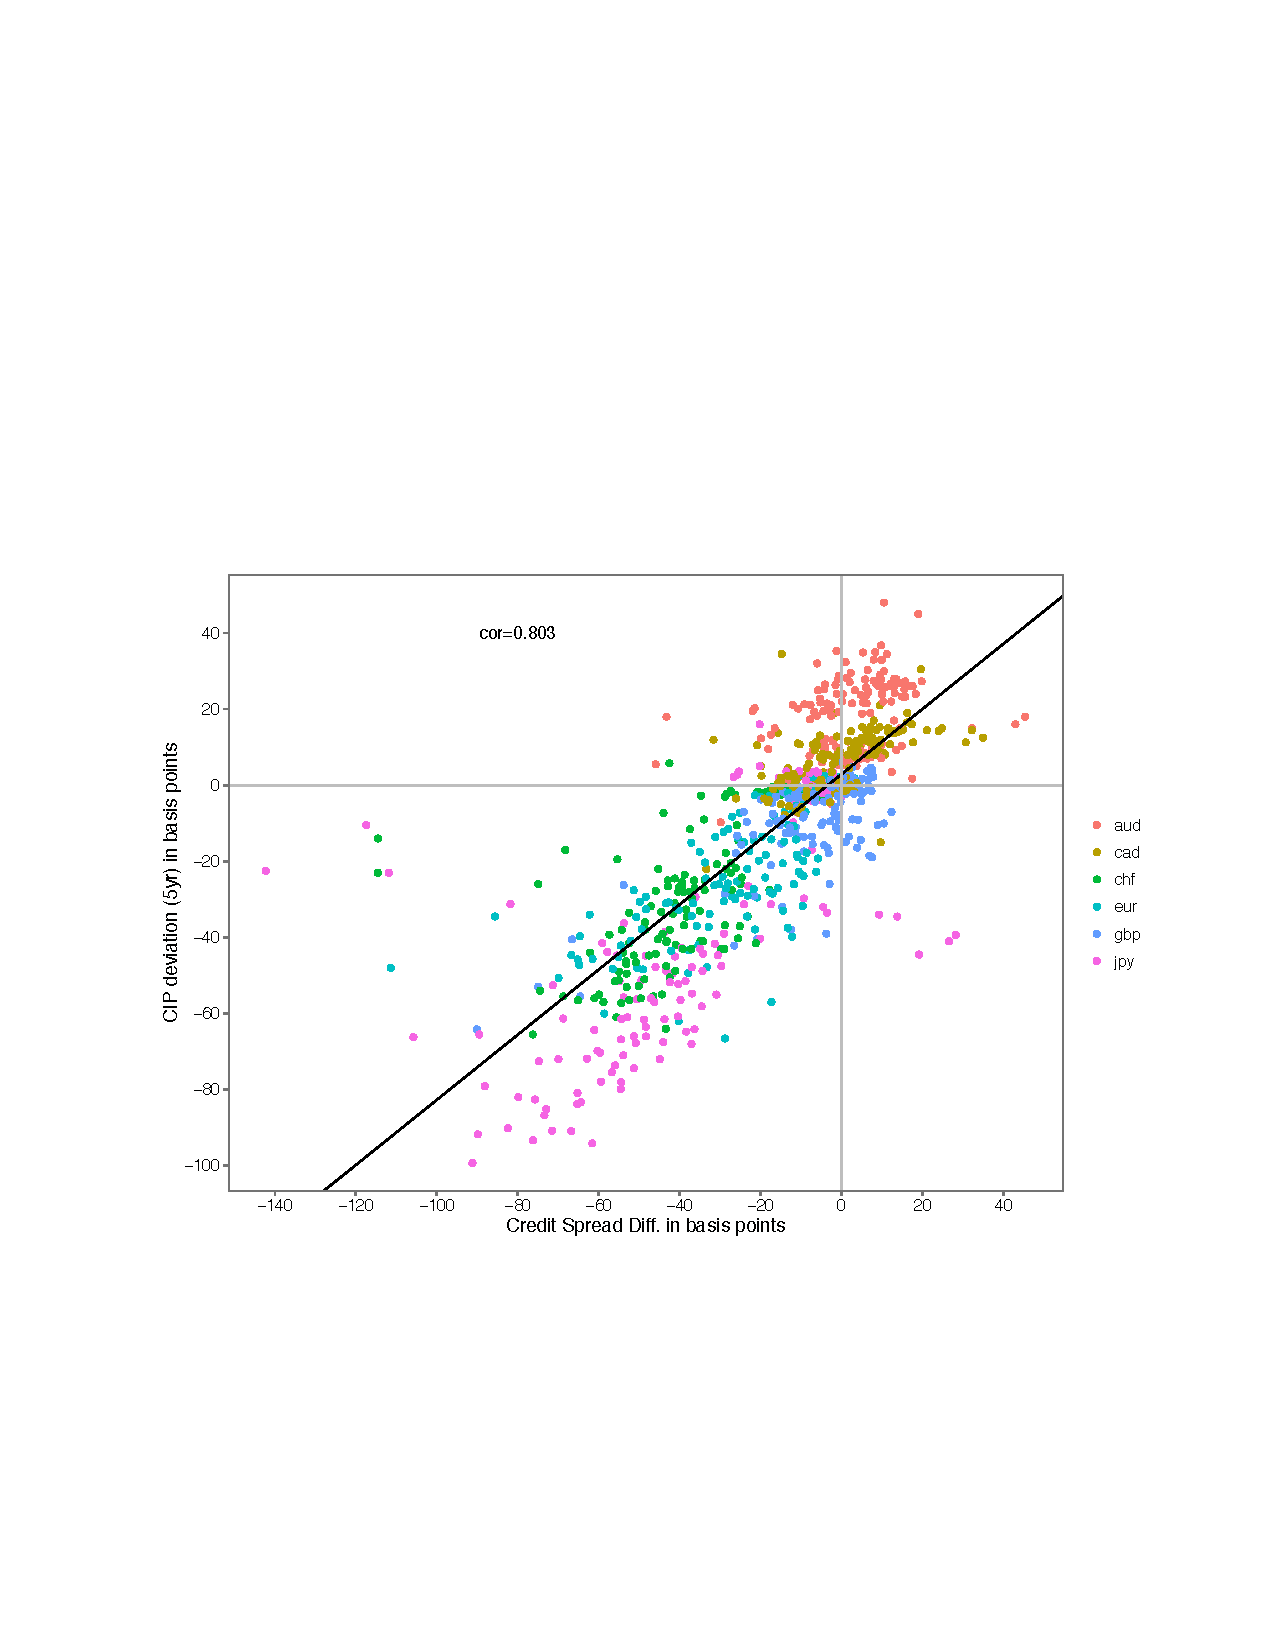
\includegraphics[height=3.1in]{images/Liao2016Figure5_orig}
\newline 
 Note: {\small Plots of CIP basis against residualized credit spread differential, for all currencies.  Panel A is from this work and Panel B is from Liao's.  The red-dashed trend line in Panel A is from a linear regression.  Liao did not document what the black line was in his plot.}
\newline \noindent Source: (Panel B only) Liao(2016)\cite{Liao2016}
\end{figure}



\section{Alternative Interest Rate} \label{govt_chapter}

Liao's study, as well as others in the field, uses the swap rate instead of a government bond rate to compute the CIP basis.  This section presents reasons why this may not be good practice and then reproduces the results of Section~\ref{Liao_chapter} using government bond rates as the reference rate.

\subsection{Reasons Not To Use the Swap Rate} \label{not_swap_section}

% The swap rate is not an interest rate.  That is, there exist bonds with the same risk and duration with lower prices or, equivalently, higher yields.  In this section, I'll define the swap rate, explain why it is not an interest rate, and provide some small evidence that it is not acting like an interest rate in practice.

Swap rates are convenient to gather and use in calculations of CIP basis, but there are a number of reasons why swap rates may not be appropriate.  Two reasons are presented in this subsection.  The first applies to all bank borrowing rates (i.e., including LIBOR and OIS), and not just the swap rate.  

% Du et al. in footnote 5\cite{Du2017} credit Frenkel and Levich\cite{Frenkel1975} for this practice.

CIP requires the bonds involved to have the exact same risk.  Banks from different countries have different default risks and the bank borrowing rates (OIS and interbank loans) will reflect those different risks.  While the financial systems of countries are linked, they do not move identically.  If a trader goes long USD LIBOR and short EURIBOR, they are not left with zero risk. 

% I think I already made this point
%Even if the risks were different, the calculation of CIP basis would be the same if the bank borrowing rates all had the same spread over the risk-free rate.  This is not the case.  Crises in individual countries happen, affecting the rates.  \todo{examples?  data?}

Experimentally, Frenkel and Levich\cite{Frenkel1975} found that CIP basis calculated with interbank loan rates was generally closer to zero than when CIP basis was calculated with government bills.  This may be because banks are more likely to increase borrowing (i.e., go short) in order to exploit currency prices than governments are.  But if that condition held before the crisis, it does not necessarily mean it will hold during the crisis.\footnote{In fact, Frenkel and Levich chose to measure CIP basis during a calm period: ``The empirical analysis covers the period between January 1962 and November 1967. The choice of the period was determined by our preference for a relatively ``quiet period" which was terminated by the British devaluation.''\cite{Frenkel1975}}


The second reason not to use swap rates is that swaps are not bonds.  Treasury notes, OIS and LIBOR are all loans for a fixed amount of money, but an interest rate swap is a contract for an exchange of floating payments.  

Unlike the market for U.S. Treasuries, where customers are trying to buy bonds, the market for interest rates swaps has customers who are trying to buy a contract, most often to be part of a portfolio with other securities (e.g., to hedge risk).  Because the customers are interested in particular portfolios, not the contract by itself, it is not clear from the contract's definition what the price in the market should be.  In fact, the prices of interest rate swaps have been studied\cite{Jermann2017} because, since 2009, the 20Y swap rate has spent most of its time below the 20Y U.S. Treasury bond rate, which many found to be unexpected.  (See Figure~\ref{swap_vs_govt}.)

\todo{Decide if I want 30Y or 20Y in the above paragraph.  The figure referenced is for 20Y.}

The interest rate swap is equivalent to exchanging a fixed-rate bond for a variable-rate one.  For USD swaps, the variable-rate bond uses the LIBOR 3M rate and, for EUR swaps, the variable-rate bond uses EURIBOR 3M.  Other authors measure CIP basis by the difference between the USD and EUR interest rate swap rates, which means they are measuring the difference between payments of LIBOR 3M and EURIBOR 3M.  It is not obvious why these should have equal risk or even have equally priced risk.  This argument is strengthened by larger spreads between OIS and the interbank loan rate since the crisis.\cite{Du2017,Borio2016}

% Even if true, what does this add to the argument?
%Interest rate swaps will have increasing error for long horizons.  An interest-rate swap that lasts for 3 months has 1 variable-rate period and is equivalent to LIBOR.  A swap that runs for 6 months has 2 variable-rate periods.  It is equivalent for investing the month for 3 months and then investing the money for 3 more months.  But the swap contract does not consider investing the money for the whole 6 month period.  Longer investment has traditionally brought higher interest rates for the same level of risk.  Thus, the variable-rate leg of the swap contract isn't maximizing its value and the rate for long-term swaps is unlikely to reflect the real price of a loan with that investment horizon.



%That reason is that the swap rate is not an interest rate.  That is, there exist bonds in the market with the same risk and duration with lower price (or, equivalently, higher yield).\footnote{For an explanation of the arbitrage of a swap, government bond and REPO and why it is not holding, see Jermann\cite{Jermann2017}} A 30Y swap has 120 periods of LIBOR 3M loans and there exist numerous different ways those periods could be invested for terms longer than 3 months and get a better return for similar risk.  Since 2009, the 30Y swap rate has spent most of its time below the 30Y U.S. Treasury bond, despite most people considering the banks to be riskier than the U.S. government, see Figure~\ref{swap_vs_govt}.

% The LIBOR 3M rate is an interest rate.  It is a market price for that level of risk for a 3 month duration.\footnote{Technically, LIBOR is an average of the rates reported in a survey, and, therefore, not the result of the market.  This is what left it open to manipulation.\cite{DOJ}  If LIBOR is not the market rate for interest, my argument is only stronger.}

% But consider a 6M swap, which is one fixed-rate coupon for two variable-rate payments.  The variable rate side is a LIBOR 3M loan, followed by a second LIBOR 3M loan.  Is that the best allocation of capital for 6M at that level of risk?  Couldn't allocating that money for the entire 6 months to a bank get a better rate at an equivalent level of risk?  If so, then the 6M swap rate is not an interest rate.  

% That effect is larger when there are more periods.  

\todo{write paragraph on empirical results, that it doesn't behave like bank borrowing rate.  Cite Figure~\ref{swap_vs_govt}.}

\begin{figure}[p]  % h = here
\textbf{\caption{\label{swap_vs_govt} Spread of swap rate over the government rate}}
\noindent \textbf{Panel A:} \newline
\includegraphics[height=3.1in]{images/SwapVsGovt_all_2Y.eps}
\noindent \textbf{Panel B:} \newline
\includegraphics[height=3.1in]{images/SwapVsGovt_all_20Y.eps}
Note: {\small The swap rate minus the rate on government bonds, over time.  Panel A uses 2 year bonds; Panel B uses 20 year bonds.  For shorter terms, the swap rate behaves like a bank borrowing rate, staying a small amount above the government rate.  And during the crisis, when banks were under distress, the spread rose.  However, for longer terms, the swap rate does not behave like a bank borrowing rate.  It went below the government rate and, during the crisis, it dropped rather than rose.}
\newline \noindent Source: Central banks, Bloomberg L.P.
\end{figure}


%\todo{ I know Jermann has comments on arbitrage of swaps.  Need to read that an insert something here.}

% \todo{ drop paragraph on SIVs}

% But from 1988 to 2008, there might have been.  A structured investment vehicle (SIV) was a kind of financial company that borrowed money cheaply over the short term and used the funds to hold long-term bonds.  If they held high-quality bonds, they could lever their capital 14 times.\cite{Crisis2010}  At peak, SIVs held 400B USD (equivalent) in assets.\cite{Telegraph}  This ``borrow short (term), buy long (term)'' strategy would have increased the LIBOR and decreased long-term corporate rates, which would have pushed the swap rate up and market rates down, bringing them closer together.  The trading strategy failed when the crisis hit, because many high-quality bonds were downgraded, short-term rates spiked, and long-term rates fell.  The last SIV defaulted in Oct.\ 2008.\cite{FT_SIV, Reuters}  

%Late in 2008, swaps of all durations fell by close to 1 percentage point relative to U.S. Treasuries.\cite{Jermann2017} The 30Y swap went below the U.S. Treasury and has stayed there for most of the time since then.  This is only anecdotal evidence --- I have not shown a connection and there certainly were other significant events in finance at the time.  Unfortunately, I did not have more time to devote to this topic.

% Prior to 2007, CIP held for swap rates which made it good for comparisons between currencies.  In fact, it held tighter than for government bonds.  (Compare Figure~\ref{CIP_basis_govt} with Figure~\ref{CIP_basis_swap}.)  However, after 2008, it has not.

Multiple papers in the CIP field use swap rates for their long-term rates.  Borio et al.\cite{Borio2016} use them.  Others use a variant, the ``cross-currency basis swap'', which is two interest rate swaps packaged together.  Those appear in Liao\cite{Liao2016}, Du, et al.\cite{Du2017} and Avdjiev et al.\cite{Avdjiev2016}.  

\todo{summary sentence at the end of this?}

\todo{Where do I play off the bad parts of govt rates?}


%Avdjiev2016, page 2, Figure 1, ``cross currency basis swap spreads''
%Borio2016, page 50, Box B, ``interest rate swap rate''
%Coffey2009 --- NO PROBLEM ---used 3 month graphs with LIBOR or TBill
%Du2017, --- Page 11, "cross currency basis swap" (floating rate EUR for floating rate USD + fixed).  PROBLEM IS MITIGATED BY ALSO USING  Bund, but also uses "tenor basis swap", which swaps 3M LIBOR for 1M LIBOR + fixed basis payment.  
%Rime2017,  --- NO PROBLEM --- short time only



\subsection{Results Using Government Bond Rates}

I reproduced Liao's work using government bond rates, instead of the swap rates.  In this subsection, I describe the changes to the analysis and the results.

\todo{the first sentence of the next paragraph (especially ``exactly'') is strange.}

The set of bond prices used is not exactly the same as in the previous section's study.  The regression requires the spread of the bond rate over the reference interest rate.  In the previous section, the reference rate was the swap rate and, in this section, it is the government rate.  When the reference rate for a particular date does not exist, the data sample was dropped.  Missing swap rates happened occasionally, with no particular pattern.  With government rates, it was more systematic.  (See Table~\ref{govt_maturities}.)  For example, AUD and NZD do not have 20 year bonds; their maximum is 10 years.  So, for those currencies, only data within 10 years of the measured date was used.

\begin{table}[H]
\caption{\label{govt_maturities} Maturities priced by central banks
}
\centering
\begin{tabular}{ |l|r|r|r|r|r|r|r| }
\hline
Currency & 1-year bond & 2Y & 3Y & 5Y & 7Y & 10Y & 20Y \\
\hline
USD & Y & Y & Y & Y & Y & Y & Y \\  
EUR & Y & Y & Y & Y & Y & Y & Y \\  
JPY & Y & Y & Y & Y & Y & Y & Y \\ 
CHF & Y & Y & Y & Y & Y & Y & Y \\ 
GBP & Y & Y & Y & Y & Y & Y & Y \\ 
AUD &   & Y & Y & Y &   & Y &   \\ 
CAD & Y & Y & Y & Y & Y & Y & Y \\ 
SEK & Y & Y &   & Y & Y & Y &   \\ 
NOK & Y &   & Y & Y &   & Y &   \\ 
NZD & Y & Y &   & Y &   & Y &   \\ 
\hline
\end{tabular}

\raggedright 
 Note: {\small Central banks estimate prices for their country's bonds in the secondary market.  `Y' indicates that the maturity is priced by the central bank.}
\newline Source: Central banks
\end{table}

The goal of replacing swap rates with government rates was to obtain greater accuracy, not to improve the correlation.  But the correlations of the pooled sample did improve from 68\% to 82\%.   Table~\ref{govt_correl_table} has separate correlations for each currency.  


\begin{table}[H]
\caption{\label{govt_correl_table} Correlation of RCSD with CIP basis using govt. rates}
\centering
\begin{tabular}{ |l|r|r|r| }
\hline
Currency & Govt. Correlation & Swap Correlation & Liao's Correlation \\
\hline
EUR & .85 & .85 & .77 \\
JPY & .44 & .57 & .72 \\
CHF & .45 & .67 & .71 \\
GBP & .56 & .18 & .74 \\
AUD & .91 & .47 & .28 \\
CAD & .90 & .19 & .57 \\
SEK & .82 & .53 & N/A \\
NOK & .87 & .77 & N/A \\
NZD & .79 & .53 & N/A \\
all currencies & .82 & .68 & .81 \\  % Liao value from the bottom of page 2.
\hline
\end{tabular}

\raggedright 
 Note: {\small Correlation of RCSD with CIP basis using government bond rates with a 5-year horizon.  The row ``all currencies'' reflects a pooled sample containing the 9 currencies in my data and 6 currencies in Liao's.  (Liao did not study SEK, NOK, nor NZD.)}
\end{table}


Figures~\ref{Govt_EUR} to~\ref{Govt_NZD} show the residualized credit spread differential and CIP basis using government rates in Panel A and swap rates in Panel B.  The CIP basis has a 5-year horizon.  The error bars in all plots are the 95\% confidence interval computed using robust standard errors clustered at the firm level.


In general, the separation of RCSD and CIP basis is similar between the pairs of plots. Some features of Figures~\ref{Govt_EUR} to~\ref{Govt_NZD} are:
\begin{itemize}

\item In all plots using government rates, the CIP basis from 1998 to 2007 is farther from the x-axis when using government rates than when using swap rates.  Swap rates are generally within 30bp of the x-axis, while government rates can exceed 60bp, such as with EUR in 1999.  The distance between CIP basis and RCSD seems similar to the plots using swap rates.

\item Just as with the swap rate data, there were dramatically fewer bond prices for the time from May 2002 to July 2005.  In plots of EUR, JPY and CHF (Figures~\ref{Govt_EUR} to~\ref{Govt_CHF}), this is the likely cause of the higher standard errors in RCSD from mid-2002 to late 2004.  For CAD, SEK, and NZD (Figures~\ref{Govt_CAD}, \ref{Govt_SEK}, and~\ref{Govt_NZD}), this is the likely reason why no value for RCSD was able to be computed for periods between early 2003 to late 2005.
There were fewer than 900 price sample in each month from May 2002 to July 2005.  (Every month in 2000 and 2001 exceeded 1,300 samples.  As did every month after January 2006, excepting holidays.  See Table~\ref{price_samples}.)  


%in all government plots, RCSD shows higher standard errors from May 2002 to July 2005.  This is because there were fewer price samples in the data set.  Of note is CAD in Figure~\ref{Govt_CAD}, which has prices for just one bond for February and March of 2004.  A similar effect can be seen with NOK in Figure~\ref{Govt_NOK}, which has prices for just one bond from Dec. 2001 to April 2002.  

\item Just as with the swap rate data, for EUR in Figures~\ref{Govt_EUR}, the value of RCSD is significantly below CIP basis for most of 2003.  This could be due to the few price samples in the data set.  The closest historical events are in 2002: EUR coins and notes were issued and Greece joined the Eurozone.  

\item Just as with the swap rate data, in most plots there is a steep drop in both RCSD and CIP basis in late 2008 and early 2009.  This is related to the Global Financial Crisis and, for CIP basis, signals that it was more profitable to invest domestically than in the U.S\@.  In November 2008, the U.S. Federal Reserve System started the quantitative easing later known as ``QE1''.  

\item Just as with the swap rate data, for JPY (Figure~\ref{Govt_JPY}), there was a rise in RCSD without a rise in CIP basis from mid-2009 to mid-2010.  The Global Financial Crisis had a dramatic effect on Japan, but it rebounded with 4.2\% growth in 2010, as compared to America's 2.5\% and the E.U.'s 2.0\%. 

\item Just as with the swap rate data, for GBP (Figure~\ref{Govt_GBP}), RCSD was significantly above CIP basis from late-2011 to mid-2013.  During the same period, for NOK (Figure~\ref{Govt_NOK}), RCSD was significantly below CIP basis.  This is during the peak of the Euro debt crisis, where the yield for Greece's long-term debt went above 25\% and Portugal's above 13\%.  The United Kingdom is part of the E.U., but does not use the Euro currency.  Norway is not a member of the E.U., but is part of the European Economic Area, which has free movement of persons, goods, services, and capital (the ``European Single Market'').  

\item Just as with the swap rate data, for some graphs, the CIP basis is significantly above or below the RCSD from 2013 onward.  EUR, AUD, NOK has it above and JPY has it below.

\end{itemize}



\todo{Descriptions are too casual and too vague.  Needs statistics.}

% Figure~\ref{Govt_EUR} has the plots of EUR.  In both, the residualized credit spread differential stays close to the CIP basis.   The most notable feature is that the RCSD and CIP basis using government rates are not close to zero prior to 2008, while those computed with swap rates are.  This effect is seen, to some degree, in all of the plots of government rates in this section.

% \todo{Compute a scale for CIP basis swap and govt prior to 2007.  Mention it here.}

% Figure~\ref{Govt_JPY} has the plots of JPY.  In both plots, RCSD and CIP basis appear to be uncorrelated from mid-2008 to mid-2010.  Similar to EUR and the other graphs, prior to 2008, RCSD and CIP basis using goverment rates depart much farther from zero than those values calculated with swap rates.  

% \todo{quantify distance from x-axis prior to 2008}

% \todo{measure correlation outside 2007-2010 ?}

% Figure~\ref{Govt_CHF} has the plots of CHF.   With government rates, RCSD and CIP basis move together, except at a few extreme points in late 2008 and early 2009. 

% \todo{Find history and assign events to each of these dates.}
 
% Figure~\ref{Govt_GBP} has the plots of GBP.  Using government rates, the RCSD follows CIP basis more closely during the extremes of 2008 and 2009.  

% Figure~\ref{Govt_AUD} has the plots of AUD.  Using government rates, prior to 2008, the CIP basis is mostly within the 95\% confidence interval of the RCSD.  However, when using swap rates, the CIP basis is significantly above from 1999 to 2004. 

% Figure~\ref{Govt_CAD} has the plots of CAD.  The plots using government rates vary more than those using swap rates, but otherwise the plots of RCSD and CIP basis mostly overlap.

% \todo{Address data in CAD 2004!}

% \todo{Can I say ``overlap'' more quantitatively??}

% Figure~\ref{Govt_SEK} has the plots of SEK.  For both government and swap data, the CIP basis remains mostly inside the 95\% confidence interval, even during the extremes of late 2008 and early 2009.  
 
% Figure~\ref{Govt_NOK} has the plots of NOK.   

% \todo{Any description of NOK?}

% \todo{Address data in NOK 2002!}
 
% Figure~\ref{Govt_NZD} has the plots of NZD.   RCSD using the government graphs follows CIP basis during the extreme movements of late 2008.  Those movements are not present in the CIP basis when calculating swaps. 

Figure~\ref{Govt_XY} has comprehensive results, a plot of CIP basis against RCSD.  Panel A contains results using government rates as the reference rate and Panel B contains results using swap rates.

Government rates were used to get better accuracy, not a higher correlation.  But the correlation did improve and the trend line in Figure~\ref{Govt_XY} improves as well.  The slope is closer to 1 (from .6390 to .9039) and a higher r-squared (from .4890 to .7222).

\todo{probability slope is 1 and constant is 0}


\clearpage

\todo{ remove page break}


% currency, note
\newcommand{\comparegovtfig}[2]{
\begin{figure}[H]  % h = here
\textbf{\caption{\label{Govt_#1} Residualized credit spread diff. of #1}}
\noindent \textbf{Panel A:} \newline
\includegraphics[height=3.1in]{images/Liao2016Figure4_#1_govt}
\noindent \textbf{Panel B:} \newline
\includegraphics[height=3.1in]{images/Liao2016Figure4_#1_xcbs} 
Note: {\small Panel A uses government rates and Panel B uses swaps.  The RCSD is plotted in blue (dotted) with the 95\% confidence interval in gray.  CIP basis is in red (solid). #2}
\newline \noindent Source: Central banks, Bloomberg L.P. 
\end{figure}
}


\comparegovtfig{EUR}{}
% The government plot shows a reverse story --- instead of CIP breaking in 2007, it did not hold from 1998 until 2012.

\comparegovtfig{JPY}{}
% These plots are similar, except the government one seems a little lower.

\comparegovtfig{CHF}{}
% These graphs are similar, except the government one seems a little lower.

\comparegovtfig{GBP}{}
% These graphs differ, but the closeness of the credit spread differential to the CIP seems roughly the same

\comparegovtfig{AUD}{}
% While the swap-rate plot is relatively flat, the government plot moved around.  In both, the credit spread differential is always close to the CIP.

\comparegovtfig{CAD}{}

\comparegovtfig{SEK}{}

\comparegovtfig{NOK}{}

\comparegovtfig{NZD}{}



% X-Y plots 

\begin{figure}[H]  % h = here
\textbf{\caption{\label{Govt_XY} CIP basis vs. RCSD}}
\noindent \textbf{Panel A:} \newline
\includegraphics[height=3.1in]{images/Liao2016Figure5_govt_alldata}
\newline 
\noindent \textbf{Panel B:} \newline
\includegraphics[height=3.1in]{images/Liao2016Figure5_xcbs_alldata}
\newline 
Note: {\small Plots of CIP basis against residualized credit spread differential.  Panel A is with government bonds yields as the reference rate; Panel B with swap rates.  The red-dashed trend line in both plots comes from a linear regression.  Using government rates results in a slope that is closer to 1 and a higher r-squared.  }
\newline \noindent Source: Central banks, Bloomberg L.P.
\end{figure}


\section{Measuring Corporate CIP Basis} \label{corp_cip_chapter}

So far, this work has measured CIP basis using swap rates and government bond rates.  In this section, I present a different approach: using corporate bond prices.  First, the model used for the measurement is described and its assumptions are discussed.  Next, details are discussed which are necessary for applying the model to real data.  Then, the model is compared and contrasted with Liao's regressions and work by Du et al.  Lastly, the results are plotted and compared to CIP basis data gathered from swaps and government rates.  

\subsection{Corporate Bonds for CIP}

Measuring CIP basis requires bonds, issued in different currencies, with the exact same risk.  Government bonds can be used only if we assume that they are all risk-free.  This is a plausible assumption, but a questionable one since only 3 of the 10 governments (Germany, Switzerland, and Norway) were top-rated by all three major credit rating agencies (S\&P, Moody's, Fitch) for the period of this study, from Jan.\ 1998 to March 2017.\cite{TradingEconomics}  Swap rates, as detailed in Section~\ref{not_swap_section}, are not bonds and do not have the same risk.  However, corporate bonds issued by the same firm in multiple countries should have similar risks.

\todo{present ratings of government bonds}

Bonds issued by the same firm in multiple countries are not identical.  Their prices can be affected when they are traded in different markets, with different ticksizes and different bid-ask spreads.  Financial markets can differ because of each country's policy on inflation.  In the case of default, depending on how bonds are issued, different countries have different courts and legal policies.  Some countries might bailout native firms, but not foreign firms.  And large international defaults can become political events.  

Corporate bonds also differ in their attributes.  A corporation can issue bonds with different maturities, different coupons, etc.  In this section, I assume that the risk of a corporate bond does not depend on the currency it is issued in.  However, bonds with different maturities will be allowed to have different levels of risk.  That risk will be accounted for, when bond prices are used to measure CIP basis.

% Is this needed?  I don't think so now.
%A separate but related question is whether or not CIP should hold at all for bonds that do not have the same maturity.  CIP should hold for corporate bonds with the exact same risks, but a 4-year USD bond and a 6-year EUR bond do not have the same risks.  When performing a trade to short the 4-year USD and go long the 6-year EUR, the Sharpe ratio will not be infinite.  Nonetheless, the risks are very similar, especially over the near term that might concern an arbitrageur who has to hold the position (or bank that loans against it).  Thus, CIP should hold for corporate bonds of similar, if not exact, maturity.



\subsection{Model} \label{corp_cip_model}

The model assumes that there are many corporations, each with bonds giving a (potentially) different measure of corporate CIP basis.  To resolve these different values, the model presumes there is a ``true'' CIP basis and there is some error in each measurement.  Below, I'll present the model for a bond's yield, the model's assumptions, and then justify that the model accurately reflects the definition of CIP basis.

% Model
The model is defined in terms of a bond's yield so that CIP basis will be consistent when there are more than 2 currencies.  The bond's yield is:
\begin{equation}
  \label{first_model}
 y_{f,c} = \log\left(\frac{S_{c,USD}}{F_{c,USD}}\right) - b_{c} + \zeta_{f} + \epsilon_{f,c} 
\end{equation}
% Definitions and assumptions

\todo{claim this equation does embody CIP basis for a single-firm case}

\noindent where $y_{f,c}$ is the yield of a bond from firm $f$ in currency $c$, $S_{c,USD}$ is the spot exchange rate for currency $c$ in USD, $F_{c,USD}$ is the forward exchange rate, $b_{c}$ is the CIP basis for currency $c$ with USD as the reference currency, and $\zeta_{f}$ is the true yield for a bond from firm $f$ in USD.  Recall that CIP basis is in relation to a specific time horizon, such as 5 years, so the forward's delivery date and bond's maturity must share that same horizon.

The assumptions for this model are that $\epsilon_{f,c}$ are i.i.d., that $\E[\epsilon_{f,c}] = 0$, and that $\Var(\epsilon_{f,c}) = \sigma_{f,c}^2$.  For yields, $y_{f,c}$ are i.i.d.\ and $\E|y_{f,c}|$ is finite.  For $\zeta_f$, I assume $\E[\zeta_f]$ is finite and that $\E[\zeta_f]$ does not change if the set of firms is restricted by the currencies in which the firms issue bonds.

% Economic rationale for assumptions

These assumptions are not ideal, but are practical.  The $\epsilon_{f,c}$ terms represent the error of pricing the bonds by the market.  Assuming the firms' errors are uncorrelated between firms is unrealistic in practice, since there exists sectors in which firms' revenues are correlated.  Nonetheless, many other stock and bond analyses make (or accept) the assumption that different firms have unrelated profitability, as is done here.  

There is potential for selection bias in the model, since firms use bond yields to decide in which currencies to issue bonds.  Bonds might not exist in currencies with high yields because firms choose the currency with the lowest yield in which to issue.  This effect is lessened by using prices from the secondary market.  

The selection bias does not affect $\zeta_f$ directly, but may do so indirectly.  There is no direct effect because a firm's profit from issuing a bond overseas is affected by the CIP basis, $b_{c}$, and not by its true yield in USD, $\zeta_f$.  That is because, in the model, the true yield has the same effect on all markets.  There is an indirect effect because larger firms are more likely to have a low $\zeta_f$ and more likely to have lower overhead for issuing overseas bonds.  Thus, there might be correlation between issuance and $\zeta_f$.  Since the data is limited to bond issues of 150M USD (or equivalent), I assume all firms issuing are large and the selection bias does not affect $\zeta_f$.

\todo{Dad says: too terse above.}

% ? Test numbers with recently-issue bonds vs. older bonds that aged into that maturity?

% Show this model matches definition of CIP

\todo{when addressing single-firm case, the sentence below should be modified}

For this model, its estimate of CIP basis can be computed by averaging and its result is consistent with the definition of CIP basis.  To derive this, take the mean of the yield over firms 1 to $\phi$ to get:
\begin{equation}
\frac{\sum_{f=1}^{\phi} y_{f,c}}{\phi} =  \log\left(\frac{S_{c,USD}}{F_{c,USD}}\right) - \hat{b}_{c} 
+ \frac{\sum_{f=1}^{\phi} \zeta_{f}}{\phi} 
+ \frac{\sum_{f=1}^{\phi} \epsilon_{f,c}}{\phi}
\end{equation}

\noindent Letting $\phi$ go to infinity, by the Law of Large Numbers, we get:
\begin{equation}
 \E[ y_{f,c} ] =  \log\left(\frac{S_{c,USD}}{F_{c,USD}}\right) - \hat{b}_{c} 
+ \E[ \zeta_{f} ]
+ \E[ \epsilon_{f,c} ]
\end{equation}

\noindent Using the assumption $\E[ \epsilon_{f,c} ]=0$ and solving for $\hat{b}_{c}$ we get:
\begin{equation}
  \label{first_zeta}
\hat{b}_{c} = \log\left(\frac{S_{c,USD}}{F_{c,USD}}\right) + \E[ \zeta_{f} ] - \E[ y_{f,c} ]
\end{equation}

\todo{!!!! Saroj wanted multi-line paragraphs indented?}

Now, if $c$ is USD, there is no exchange of currencies and the CIP basis is by definition 0, yielding:
\begin{equation}
  \label{second_zeta}
\E[ \zeta_{f} ] =  \E[ y_{f,USD} ]
\end{equation}

\noindent Using equation~\eqref{second_zeta} to substitute $\E[ \zeta_{f} ]$ in equation~\eqref{first_zeta}, we get:
\begin{equation}
 \hat{b}_{c} = \log\left(\frac{S_{c,USD}}{F_{c,USD}}\right) + \E[ y_{f,USD} ] - \E[ y_{f,c} ] 
\end{equation}

\noindent Using the approximations $e^x \approx 1+x$ and $\log(1+x) \approx x$ for small $x$, we get:
\begin{equation}
 \hat{b}_{c} \approx \frac{S_{c,USD}}{F_{c,USD}}(1 + \E[ y_{f,USD} ]) - (1 + \E[ y_{f,c} ]) 
\end{equation}

% Derivation of above formula:
% b_{c} = \frac{S}{F}e^{r_{c'}} - (1 + r_{c})
% b_{c} + (1 + r_{c}) = \frac{S}{F}e^{r_{c'}}
% \log(b_{c} + (1 + r_{c})) = \log\left(\frac{S}{F}e^{r_{c'}}
% b_{c} + r_{c} = \log\left(\frac{S}{F}\right) + r_{c'}
% b_{c} = \log\left(\frac{S}{F}\right) + r_{c'} - r_{c}

\todo{dad: expand this}

\noindent Which is analogous to the definition of CIP basis:
\begin{equation}
 b_{c} = \frac{S_{c,USD}}{F_{c,USD}}(1 + r_{USD}) - (1 + r_{c}) 
\end{equation}

\todo{the intro sentence below is awkward}

The model has been presented and justified to represent the definition of CIP basis.  Next, I'll go into the details of applying the model to real-world aspects of the data.

\subsection{Adjusting Yields} \label{adjusting_yields} 

% May want to think more about how to adjust yields and what arbitragers do.
% !!! Need to mention that government bond rates are, themselves, estimates!

The model in equation~\eqref{first_model} assumes that every firm has multiple bonds that mature exactly with the CIP basis's horizon.  That is, when calculating the CIP Basis with a 5-year horizon, the bonds all mature in exactly 5 years.  This is rarely the case.  When analyzing the data, the bond yields must be adjusted so that they estimate the yield of a 5-year bond, even if they happen to be a 4- or 6-year bond.

The adjustment is done by calculating the spread of the corporate bond over a government bond and then applying that spread to a government bond with the horizon's maturity.  For example, if we want the yield of a corporate bond with a maturity of 5 years in EUR, but have a bond with a maturity of 4 years, we start by finding the yield of a government bond of 4 years.  If none exists, we do a linear interpolation of the yield from the nearest government bonds, in this case, the 3- and 5-year German bund.  If the estimated 4-year German bund has a yield of 1.0\% and the 4-year corporate bond has a yield of 3.2\%, we subtract to get the spread of 2.2\%.   To get our estimate of the 5-year corporate bond rate, we add that spread to the rate of the 5-year German bund.  If that was 1.1\%, the estimated corporate rate would be 1.1\% + 2.2\% = 3.3\%.  

In the following discussion, the term ``adjusted yield'' refers to a bond's yield that has been adjusted by this process to reflect a maturity equal to the CIP's horizon.  It should be obvious that the maturity cannot be adjusted too far without a loss of quality to the estimate.  When targeting a CIP with a 5-year horizon, only bonds with a remaining maturity between 3 years and 7 years were used.  

% Table of all maturity windows ?

This adjustment includes an additional source of error that comes from the government rates.  The government rates are estimates themselves.  They are assembled by the central banks from secondary market prices for government bonds.  That means, the 5-year government rate may be an estimate from government bonds that themselves have maturities shorter or longer than 5-years.  In the process of adjusting corporate yields, the government rate is both added and subtracted and the rates chosen are close in maturity, so its effect should be small.

\subsection{Multiple-bond Model}

The model in equation~\ref{first_model} assumes that firms issue at most one bond per currency, but in reality, there may be many.  In this subsection, the single-bond model is modified.  The important change is that errors are allowed to be correlated for bonds that share the same currency and firm.  

\todo{!!!!! Saroj asked ``what does the above sentence mean''}

The model for a bond's yield becomes:
\begin{equation}
  \label{second_model}
 y_{f,c,i} = \log\left(\frac{S_{c,USD}}{F_{c,USD}}\right) - b_{c,USD} + \zeta_{f} + \epsilon_{f,c,i} 
\end{equation}
% Definitions and assumptions

\noindent where $y_{f,c,i}$ is the yield of bond $i$ from firm $f$ in currency $c$.  The terms $S_{c,USD}$, $F_{c,USD}$, $b_{c,USD}$, and $\zeta_{f}$ remain unchanged.  The error term $\epsilon_{f,c,i}$ is now also indexed by the bond identifier $i$.   As in the original model, the CIP basis is in relation to a specific time horizon, such as 5 years, so the future and every bond's maturity must share that horizon.

Assumptions for the model include that $\epsilon_{f,c,i}$ are i.i.d.\ and that $\E[\epsilon_{f,c,i}] = 0$.  The assumption that changes for $\epsilon_{f,c,i}$ is that $\E(\epsilon_{f,c,i}\epsilon_{f',c',i'}) = \sigma_{f,c}^2\ind(f=f' \land c=c')$.  That is, errors are correlated for the same firm and currency.  The remaining assumptions are unchanged:  For yields, $y_{f,c}$ are i.i.d.\ and $\E|y_{f,c}|$ is finite.  For $\zeta_f$, we assume $\E[\zeta_f]$ is finite and that $\E[\zeta_f]$ does not change if we restrict the set of firms by the currencies in which they issue bonds.  

This multi-bond model is solved by averaging, similarly to the single-bond model.  The model only differs in calculating the error term, where this multi-bond model uses robust clustered standard errors, clustering on the firm.

% !!! applying to real world data (e.g., adjusting bond yields to approximate that of 5 year olds bonds)


\subsection{Comparison to Liao's Regression}

The regression equation~\eqref{second_model} looks similar to Liao's equation~\eqref{liao_regression}, so it is important to highlight the differences between this work and Liao's.

First, my regression is a measurement of a general property: CIP basis.  The result of the measurement has a number of applications.  Liao's regression result is one step in verifying a model.  He is estimating the credit spread differential and then using the correlation of that estimate with CIP basis (using swap rates) to verify his model.  

Second, my regression is derived from the formula for CIP basis.  Liao's regression appears to originate from an industry practice, ``matrix pricing'', to approximate the credit spread.  His paper states, ``This method of attribution is analogous to the standard industry practice of matrix pricing in which a bond with unknown prices is assessed against other bonds with similar maturity and rating.''  The section where the regression is explained is entitled ``Matrix pricing of corporate credit'' and I could find nothing further about other origins of the regression formula.

Third, my regression has a specific time horizon.  If that horizon is 5 years, the delivery dates of forwards are in 5 years and the yields of bonds are adjusted to 5-year maturities.  Liao's regression operates on all maturities at once.  He uses maturity buckets, so a 4-year bond is treated exactly the same as a 6-year, because they are in the same bucket.  The maturity buckets are not indexed by currency, so the spread between short-term bonds of different currencies must be the same as the spread between long-term bonds of the same currencies.

Fourth, the set of assumptions is different.  My analysis assumes that the spread between a 4-year and a 5-year government bond is nearly the same as between a 4-year and 5-year corporate bond, in the same currency.  Liao's regression assumes that the spread for maturity does not depend on the currency.  It also assumes that the spread for rating does not depend on the currency, nor on the maturity.  Notice that my regression does not rely on a bond's rating, since the firms attributes are already assumed to be in the $\zeta_f$ term.

There are similarities.  Liao defines ``net deviation'' as equal to the residual credit spread differential minus the CIP basis using swaps.\footnote{Page 29 of Liao\cite{Liao2016} describes an improvement to the calculation of net deviation.  Instead of computing RCSD by regression and then subtracting CIP basis, the value for CIP basis is moved into the regression and the horizon of the CIP basis is selected to match the maturity of the bond.  This does not change any of the arguments made in this section.}  That value is very similar to the CIP basis using corporate bonds.  (See Appendix~\ref{net_deviation_data}.)  Liao assumes that net deviation should be close to 0, and converts that into a test that the credit spread differential and CIP in swap rates have a high correlation.  However, net deviation is not CIP basis.  It does not have a horizon and it assumes maturity's effect on yield is the same for all currencies.

% in model, net deviation is how firms decide where to issue
% in model, net deviation is zero with infinite corporate issuance 
% in reality, net deviation is correlated with corporations issuances
% should address pg 29 definition of net deviation
% 

% why Liao regress on firms that issued multiple currencies???  --- this is taken care of now, discussing CSD and RCSD
%Another similarity is that the regressions are limited to firms that have issued bonds in multiple currencies.  In the case of my regression, it a mathematical necessity.  CIP basis on the corporate bonds is, by definition, a difference between rates in different currencies.  Liao clearly states that ``Furthermore, the data sample is limited to only bonds belonging to multi-currency issuers.''  This is stated near the reference to ``matrix pricing'', but it is unclear why limiting data should improve the results when using matrix pricing.  

To conclude, my regression computes CIP basis from corporate bonds.  While it is similar to Liao's ``net deviation'', it is different in purpose, assumptions, and value.

%Corporations only rarely issue the same bond in multiple currencies.  It is more common for firms to have bonds in multiple currencies with different maturities.  For example, if a firm issues a 5-year EUR bond while having an outstanding 4-year USD bond.  To measure the CIP basis at the 5-year horizon, we need to adjust the yield of the 4-year USD bond to approximate what the yield would be at 5 years.  If we do this, we can then measure the CIP violation using a larger set of corporate bonds.  In practice, the Sharpe ratio for the trade that shorts the 4-year USD and goes long the 5-year EUR bond would not be infinite, but the correlations are likely to be strong enough for arbitrage traders to exploit them and hold the values close to CIP.  

%In the following discussion, I'll used ``adjusted yield'' to refer to a bond's yield that has been adjusted to reflect a maturity equal to the CIP's horizon.  In practice, a 4-year bond's yield will be adjusted to the 5-year horizon by adding the spread between the 4-year government bond and 5-year government bond.  If no 4-year government bond exists, its yield will be linearly interpolated from the closest government bonds.  Bonds will only be adjusted inside a window, for example between 3 years and 7 years for a 5-year horizon.  


\subsection{Comparison to Du et al.}

Du et al.\ also measured CIP basis using corporate bonds.  Their most detailed analysis uses bonds from a single bank.  There is also summary data from measuring CIP using bonds from supranational institutions, banks, and non-financial firms.  The details below are based on their paper and its Online Appendix.\footnote{The Online Appendix was downloaded on 10 November 2017.  On 16 November 2017, the authors were working on a revision to it.\cite{Du_email1}}

Du et al.'s work on corporate bonds centered on measuring CIP basis using bonds from a single firm: the German bank Kreditanstalt f\"u Wiederaufbau (KfW).\cite{Du2017}  The bank had a AAA rating and is owned by the German government ``with all its liabilities fully backed by the German government''.\cite{Du2017}    They analyzed bonds in the following currencies: USD, EUR, JPY, CHF, and AUD.  

The analysis used spreads over the swap rate for USD.  For KfW's bonds in USD, the ``z-spread'' was the bond's yield minus the swap rate.  For KfW's other bonds, the z-spread was the bond's yield minus both the swap rate and minus the rate of the cross-currency basis swap.  The cross-currency basis swap rate is equal to CIP basis using swap rates and was used to account for the currency conversion.   For a bond, Du et al.\ defined the ``KfW basis'' as the difference between the bond's z-spread and z-spread of a USD bond of similar maturity.

Du et al.\ computed an aggregate KfW basis for a currency, say EUR.  The first step was to group all EUR and USD bonds by maturity year.  Second, the KfW basis was computed for all pairs of EUR and USD bonds with the same maturity.  Third, the value was averaged within each maturity group.  Lastly, the average was computed across all maturities.\cite{Du_email1}   Thus, the value Du et al.\ quantified and plotted was an average of CIP basis across all horizons.

Plots of the aggregate KfW basis show some correlation with CIP basis using 3-M LIBOR.  For CHF and JPY, the aggregate KfW basis is always within 20bp of the 3-M LIBOR.    For times after the crisis, the aggregate KfW basis for all 4 currencies is generally closer to 0 than CIP basis using 3-M LIBOR.  

The authors determined that costs for the arbitrage trade were around 20 basis point and that CIP basis for the JPY, EUR, and CHF exceeded that margin for 75\%, 50\% and 30\% of the period from 1 Jan.\ 2009 to 31 Aug.\ 2016.   

%The maximum average CIP basis was AUD with 0.1bp and the minimum was JPY with -30.2bp.  

% They also estimate fees and profit with leverage, but that's not important here.

KfW is a large issuer with 370B USD (equivalent) of bonds outstanding.  However, the amount issued in both CHF and JPY was less than 5B USD (equivalent).  The authors concluded ``liquidity differential can be a potential factor in explaining the positive profits of going long in the more illiquid yen and Swiss franc KfW bonds and shorting the more liquid dollar KfW bonds.''.  But they also concluded that liquidity issues could not explain the positive spread between the USD and EUR bonds.  

% Also uses KfW-Bund spread, which is just a bank rate measurement.  Ignored it.

In addition to the analysis on KfW, Du et al.\ analyzed bonds from 16 banks and financial companies, using data gathered from Bloomberg.  The method was, presumably, the same as with KfW.  

The aggregate CIP basis was computed separately for each institution.  Each company's aggregate CIP basis reacted differently.  In 2009, one firm had an aggregate CIP basis above 150bp in AUD, while another had an aggregate CIP basis below -300bp.   All four currencies had dates in 2009 where the top and bottom firm in aggregate CIP basis were at least 400bp apart.  The plots of aggregate CIP basis were continuous; this effect did not seem to result from noise.  The firms that had extreme values for aggregate CIP basis in one currency did not necessarily have extreme values in another currency.  

The values plotted were aggregate CIP basis, which means they were an average of CIP basis at different maturities.  The maturities were not weighted evenly, because the analysis could only weight a maturity for which the firm had issued a bond and that bond had prices on Bloomberg. Also, the firms were all financial firms.  Other firms look to them to take the other side of currency transactions.  It should not be surprising that one or another might have difficulty borrowing in AUD if its clients had left it with a large position.  Unlike with KfW, Du et al.\ did not comment on issues related to the liquidity of each firm in each currency.   

\todo{!X check the item ``all financial firms'' above, because I also say non-financial firms somewhere}

Du et al.\ provides an interesting look at CIP basis for individual firms. Since individual firms only issue a few bonds, the calculation of CIP basis requires some form of aggregation across maturities to produce a meaningful number. 

\todo{summary sentence}

\subsection{Results}

% Is the order of Swap/Govt countries preserved by Corp CIP?  Can we assume the ordering is due to risk assigned to each government, not to something else?   NO.  Order is the same!
% Feb 15, 2002 has almost 0 CIP!!!
% Even post 2014, some currencies are more than 2 stdevs from CIP.
% Have some spikes pre-2007.  Probably little data?  (especially around end-2002 / start-2003)


% Plot of all Corp CIP
%   -> comment on order of countries post-2007, same as govt plot

Figure~\ref{CIP_basis_corp} contains a plot of the CIP basis inferred from corporate bond prices, for a 5-year horizon.  Figure~\ref{max_CIP_basis_spread} has the max CIP basis spread for a 5-year horizon using swap, government and corporate rates.  The abnormally low value for max CIP basis spread using corporate rates on 28 March 2016 is an Easter Monday, where 7 countries government rates were unavailable.  

\begin{figure}[h]  % h = here
\textbf{\caption{\label{CIP_basis_corp} CIP basis from corporate rates with 5-year horizon}}
\includegraphics[height=3.1in]{images/Basis_all_corp_5Y}
Note: {\small CIP basis values inferred from a corporate bond rates, using a 5-year horizon. }
%\newline Source: Bloomberg L.P.
\end{figure}

% max CIP basis spread

\begin{figure}[h]  % h = here
\textbf{\caption{\label{max_CIP_basis_spread} Max CIP basis spread}}
\includegraphics[height=3.1in]{images/BasisSpread_all_all_5Y}
Note: {\small Maximum CIP basis spread for 3 different ways of calculating CIP basis.  The gray region is the 95\% confidence interval for max CIP basis spread using corporate rates.  The max CIP basis spread is the return an arbitrageur would get when trading without leverage.  The abnormally low value for max CIP basis using corporate rates on 28 March 2016 is an Easter Monday, where 7 countries government rates were unavailable.}
\newline Source: Central banks, Bloomberg L.P.
\end{figure}

\todo{update description of figure above for confidence-interval now in plot.}


For the period from Oct. 2002 to Aug. 2004, the max CIP basis spread using corporate rates has large errors --- and even no value at all --- as a result of having few price samples in the data set.   The regression for CIP (equation~\eqref{second_model}) requirements that the bond's maturity be ``close in time'' to the horizon.  For the 5-year horizon, that was chosen to be 3 to 7 years from maturity.  In each of the Oct. 2002 to Aug. 2004 time periods, there were fewer than 200 price samples that met that requirement.  For January 2003, there were none.  Other dates outside this time periods, barring holidays, had 350 to 2100 price samples.   

From January 1998 (the start of the study) to December 2007, max CIP basis spread for the swap rate is almost flat.  It spends 90\% of its time between 10 and 25bp, with a median of 19.5.  The max CIP basis spread using government rates spends 90\% of its time between 38 and 92bp, with a median of 56.5.  Max CIP basis spread using corporate rates spends 90\% of its time between 5 and 61bp, with a median of 23.3.  The spread using corporate rates spends much of its time close to the spread using swap rates, which at that time period was the metric for measuring CIP.  The major departure from the swap rate during that time period is the Oct. 2002 to Aug. 2004 time period, which is associated with less data and higher error bounds.

From February 2009 to October 2009, max CIP basis spread is highest when computed with corporate bond rates, but this period also has larger error.  The spike is caused by a large negative movement by JPY, as seen in Figure~\ref{CIP_basis_corp}.  This spike coincided with large swings in Japanese GDP.  This spike is only seen in CIP basis calculated with corporate bonds and not when it is calculated with either government bonds nor swap contracts.  

From Mid-2011 to the end of 2012, all measures of max CIP basis spread show a peak.  This is during the height of the European debt crisis.  For CIP basis using corporate bonds, the lowest currency is usually GBP and the highest is NOK, both European Single Market currencies.  CIP basis using government bonds has JPY as its lowest and NOK as its highest.  CIP basis using swap rates has NZD as its highest and JPY as its lowest.

\todo{plot 5-year swap rates CIP!}
\todo{cite figures!}

From January 2013 to March 2017 (the end of the study), the median value of max CIP basis spread using swap rates is 96.4bp, up from 19.5bp during the 1998 to 2007 time period.  For government bonds, the median spread is 116bp, up from 56.5bp.  This is the problem that lead researchers to study CIP basis: a large bank should trade well before the spread gets to 96.4 or 116 basis points.  However, when measured using corporate rates, the median spread is 48.0 basis points.   This is roughly twice what it was before the crisis (23.3bp), but it is below the 60bp which is the believed trading threshold for banks.

\todo{!X the last sentence references 60bp as a bar for the corporate CIP basis}

CIP basis requires bonds of the same risk.  Corporate bonds from the same corporation are not identical but do have largely similar risk.  Government bonds do not have the same risk and, if that difference is significant, it can explain why the max CIP basis spread is, in general, larger when calculated using the government bonds than when calculated using corporate bonds.  

The behavior of max CIP basis spread with swaps is harder to explain.  The plots of the spread of the swap over government bonds in Figure~\ref{swap_vs_govt} show that the behavior of swaps changed during the crisis.  After the crisis, long-term swap rates moved with government rates.  This might explain why max CIP basis spread for swap rates follows the movement of max CIP basis spread for government rates.

\todo{!X  the above is vague and ``moved with'' is awful!!!}

\begin{figure}[t]  % h = here
\textbf{\caption{\label{CIP_basis_govtMinusCorp} CIP basis using govt. minus CIP basis using corp.}}
\includegraphics[height=3.1in]{images/Basis_all_govtMinusCorp_5Y}
Note: {\small CIP basis using government rates minus the CIP basis using corporate bond rates.  If CIP basis using corporate bonds is accurate, then this plot shows the price of risk for each government bond, relative to that in USD government bonds.  }
\newline Source: Central banks, Bloomberg L.P.
\end{figure}

If CIP basis using corporate bonds is an accurate measure of CIP basis, then subtracting it from CIP basis using government bonds would produce the price of risk associated with each government's bonds.  This is plotted in Figure~\ref{CIP_basis_govtMinusCorp}.  For completeness, the CIP basis using swaps minus the CIP basis using corporate bonds is plotted in Figure~\ref{CIP_basis_swapMinusCorp}.  

Notable events in Figure~\ref{CIP_basis_govtMinusCorp} are that USD (represented by the x-axis) has the highest risk bond from April 2000 to April 2002, which coincides with the March 2001 to Nov.\ 2001 recession in the U.S., and from October 2008 to March 2009, which contains the November 2008 start of quantitative easing.  JPY usually has the lowest price of risk, which is not easily explained since Japan's debt-to-GDP ratio is high for most of the time period.  But from April 2009 to October 2009, Japan has the highest price of risk, as it GDP fell and was predicted to fall at an annualized rate of -9\%.\cite{EconomistJPY2009}  

\begin{figure}[t]  % h = here
\textbf{\caption{\label{CIP_basis_swapMinusCorp} CIP basis using swaps minus CIP basis using corp.}}
\includegraphics[height=3.1in]{images/Basis_all_swapMinusCorp_5Y}
Note: {\small CIP basis using swap rates minus the CIP basis using corporate bond rates. If CIP basis using corporate bonds is accurate, then this plot shows the price of risk in swap rates, relative to that in USD swap rates. }
\newline Source: Bloomberg L.P.
\end{figure}

Figures~\ref{CIP_basis_corp_EUR} through~\ref{CIP_basis_corp_NZD} plot the CIP basis using corporate rates over time for each currency.  Also plotted are the CIP basis using swaps and CIP basis using government rates.  Some features of these figures are:
\begin{itemize}

\item In all plots, CIP basis using corporate rates shows higher standard errors or gaps from Oct. 2002 to Aug. 2004.  This is because there were fewer price samples in the data set. 

\item For JPY in Figure~\ref{CIP_basis_corp_JPY}, the CIP basis using corporate rates was a significantly not equal to 0 for all of 2009 and for most of 2012 and 2013.  Japan had a large swing downward in GDP in 2009.  But 2012 and 2013 were part of an expansionary period for the Japanese economy.  Neither seems associated with quantitative easing events, which were announced on Oct. 2010, Aug. 2011, Apr. 2013, and Oct. 2014.

\todo{!X Need citations for the above QE dates}

% lowest point for JPY in 2012 and 2013 is -55bp.  

%\item European currencies (EUR, CHF, GBP, NOK) show significant moves from 0 in CIP basis using corporate rates during 2011 and 2012, which is the peak of the European debt crisis.  However, it is hard to claim that is the cause, since SEK, another European currency, does not show similar moves and JPY, a non-European currency, does during part of that time period. 

\pagebreak 

\item For most of the time period from Jan. 2010 to the end of the study (March 2017), AUD stays significantly above zero.  Its estimate ranges from 8 to 43bp, with a median of 22bp.  

\end{itemize}


% Swap and Govt rates minus corp


\todo{Saroj has a big comment on page 83.  Not sure what it says.  Something about spacing?}

% reduce space between floats to 0
\setlength{\floatsep}{0pt}
\setlength{\intextsep}{0pt}

\begin{figure}[H]  % h = here
\textbf{\caption{\label{CIP_basis_corp_EUR} CIP basis for EUR with 5-year horizon}}
\includegraphics[height=3.1in]{images/Basis_EUR_corp_5Y}
\newline Note: {\small CIP basis values inferred from corporate bond rates are in blue (dotted), with 95\% confidence interval from clustered standard error in gray. The CIP basis calculated from government bond rates are in red (solid).  The CIP basis using swaps rates is in orange (dashed).  }
\newline Source: Central banks, Bloomberg L.P. 
\end{figure}

\begin{figure}[H]  % h = here
\textbf{\caption{\label{CIP_basis_corp_JPY} CIP basis for JPY with 5-year horizon}}
\includegraphics[height=3.1in]{images/Basis_JPY_corp_5Y}
\newline Note: {\small CIP basis using corporate rates in blue (dotted) with 95\% conf. int. in gray, using government rates in red (solid), and using swap rates in orange (dashed). }
%Note: {\small CIP basis values inferred from a corporate bond rates are in blue (dotted), with 95\% confidence interval from clustered standard error in gray. The CIP basis calculated from government bond rates are in red (solid).  The CIP basis using swaps rates is in orange (dashed).  }
\newline Source: Central banks, Bloomberg L.P. 
\end{figure}

\begin{figure}[H]  % h = here
\textbf{\caption{\label{CIP_basis_corp_CHF} CIP basis for CHF with 5-year horizon}}
\includegraphics[height=3.1in]{images/Basis_CHF_corp_5Y}
\newline Note: {\small CIP basis using corporate rates in blue (dotted) with 95\% conf. int. in gray, using government rates in red (solid), and using swap rates in orange (dashed). }
%Note: {\small CIP basis values inferred from a corporate bond rates are in blue (dotted), with 95\% confidence interval from clustered standard error in gray. The CIP basis calculated from government bond rates are in red (solid).  The CIP basis using swaps rates is in orange (dashed).  }
\newline Source: Central banks, Bloomberg L.P. 
\end{figure}

\begin{figure}[H]  % h = here
\textbf{\caption{\label{CIP_basis_corp_GBP} CIP basis for GBP with 5-year horizon}}
\includegraphics[height=3.1in]{images/Basis_GBP_corp_5Y}
\newline Note: {\small CIP basis using corporate rates in blue (dotted) with 95\% conf. int. in gray, using government rates in red (solid), and using swap rates in orange (dashed). }
%Note: {\small CIP basis values inferred from a corporate bond rates are in blue (dotted), with 95\% confidence interval from clustered standard error in gray. The CIP basis calculated from government bond rates are in red (solid).  The CIP basis using swaps rates is in orange (dashed).  }
\newline Source: Central banks, Bloomberg L.P. 
\end{figure}

\begin{figure}[H]  % h = here
\textbf{\caption{\label{CIP_basis_corp_AUD} CIP basis for AUD with 5-year horizon}}
\includegraphics[height=3.1in]{images/Basis_AUD_corp_5Y}
\newline Note: {\small CIP basis using corporate rates in blue (dotted) with 95\% conf. int. in gray, using government rates in red (solid), and using swap rates in orange (dashed). }
%Note: {\small CIP basis values inferred from a corporate bond rates are in blue (dotted), with 95\% confidence interval from clustered standard error in gray. The CIP basis calculated from government bond rates are in red (solid).  The CIP basis using swaps rates is in orange (dashed).  }
\newline Source: Central banks, Bloomberg L.P. 
\end{figure}

\begin{figure}[H]  % h = here
\textbf{\caption{\label{CIP_basis_corp_CAD} CIP basis for CAD with 5-year horizon}}
\includegraphics[height=3.1in]{images/Basis_CAD_corp_5Y}
\newline Note: {\small CIP basis using corporate rates in blue (dotted) with 95\% conf. int. in gray, using government rates in red (solid), and using swap rates in orange (dashed). }
%Note: {\small CIP basis values inferred from a corporate bond rates are in blue (dotted), with 95\% confidence interval from clustered standard error in gray. The CIP basis calculated from government bond rates are in red (solid).  The CIP basis using swaps rates is in orange (dashed).  }
\newline Source: Central banks, Bloomberg L.P. 
\end{figure}

\begin{figure}[H]  % h = here
\textbf{\caption{\label{CIP_basis_corp_SEK} CIP basis for SEK with 5-year horizon}}
\includegraphics[height=3.1in]{images/Basis_SEK_corp_5Y}
\newline Note: {\small CIP basis using corporate rates in blue (dotted) with 95\% conf. int. in gray, using government rates in red (solid), and using swap rates in orange (dashed). }
%Note: {\small CIP basis values inferred from a corporate bond rates are in blue (dotted), with 95\% confidence interval from clustered standard error in gray. The CIP basis calculated from government bond rates are in red (solid).  The CIP basis using swaps rates is in orange (dashed).  }
\newline Source: Central banks, Bloomberg L.P. 
\end{figure}

\begin{figure}[H]  % h = here
\textbf{\caption{\label{CIP_basis_corp_NOK} CIP basis for NOK with 5-year horizon}}
\includegraphics[height=3.1in]{images/Basis_NOK_corp_5Y}
\newline Note: {\small CIP basis using corporate rates in blue (dotted) with 95\% conf. int. in gray, using government rates in red (solid), and using swap rates in orange (dashed). }
%Note: {\small CIP basis values inferred from a corporate bond rates are in blue (dotted), with 95\% confidence interval from clustered standard error in gray. The CIP basis calculated from government bond rates are in red (solid).  The CIP basis using swaps rates is in orange (dashed).  }
\newline Source: Central banks, Bloomberg L.P. 
\end{figure}

\begin{figure}[H]  % h = here
\textbf{\caption{\label{CIP_basis_corp_NZD} CIP basis for NZD with 5-year horizon}}
\includegraphics[height=3.1in]{images/Basis_NZD_corp_5Y}
\newline Note: {\small CIP basis using corporate rates in blue (dotted) with 95\% conf. int. in gray, using government rates in red (solid), and using swap rates in orange (dashed). }
%Note: {\small CIP basis values inferred from a corporate bond rates are in blue (dotted), with 95\% confidence interval from clustered standard error in gray. The CIP basis calculated from government bond rates are in red (solid).  The CIP basis using swaps rates is in orange (dashed).  }
\newline Source: Central banks, Bloomberg L.P. 
\end{figure}

%\todo{add swap rate XY  plots}

% X-Y plot of govt CIP vs corp CIP 
% \begin{figure}[H]  % h = here
% \textbf{\caption{\label{CIP_basis_corp_XY} Corp. vs. Govt. CIP Basis with 5-year horizon}}
% \includegraphics[height=3.1in]{images/Basis_XY_corp_5Y}
% Note: {\small The dispersion of corporate CIP Basis is much smaller than the government CIP basis.  The correlation between them is low. }
% \end{figure}




% Table with median CIP for govt, corp, bank pre and post crisis.



% Text that could go after Corp CIP definition and before Liao's work

%The other major work using corporate bonds to study CIP was done by Liao.  

% Problematic: 
% pg 5,  "... the level of net deviation, which represents the amount of arbitragable profit,..."
% Pg 16, firm minimizes net deviation * issuance * debt    "issuance capital flow responds to the net deviation"
% Pg 20, predicts that greater net deviation will cause more overseas issuance
% Pg 21, in the limit (as more debt is issued), net deviation goes to zero

% Really a problem!!!   Pg 31
% The easiest way to construct the net deviation is to directly subtract CIP deviations from the residualized credit spread differential. However, the maturity of FX forward used for hedging each individual bond is different. To construct a measure of the net deviation, I first adjust the swap yield curve by the corresponding CIP deviation maturity curve before linearly interpolating to each individual bond’s maturity in calculating the bonds’ effective credit spreads. Then I conduct cross-sectional regression as specified in Equation 1 using this effective credit spread as the dependent variable. I take the currency fixed effects as estimates of the net deviation that corrects for maturity mismatches between FX forwards and bonds. This procedure produces estimates of c  b that is not too different from directly subtracting the 5-year CIP deviation from the credit spread differential.



% \subsubsection{CIP Basis vs. Rate}

% Du reports that firms with higher interest rates have higher CIP basis.  Is that true for CIP basis from corporate bonds?

% \begin{figure}[H]  % h = here
% \textbf{\caption{\label{BasisVsRate_govt} Government rate vs. CIP basis using govt.}}
% \includegraphics[height=3.1in]{images/GovtBasisVsRate_all_5Y}
% \newline 
% Note: {\small Plot of 5Y CIP basis, computed from government rates, against the 5Y government interest rate.   }
% \end{figure}

% \begin{figure}[H]  % h = here
% \textbf{\caption{\label{BasisVsRate_govt} Swap rate vs. CIP basis using swaps}}
% \includegraphics[height=3.1in]{images/SwapBasisVsRate_all_5Y}
% \newline 
% Note: {\small Plot of 5Y CIP basis, computed from swap rates, against the swap rate.  }
% \end{figure}

% \begin{figure}[H]  % h = here
% \textbf{\caption{\label{BasisVsRate_corp} Government rate  vs. CIP using corp.}}
% \includegraphics[height=3.1in]{images/CorpBasisVsRate_all_5Y}
% \newline 
% Note: {\small Plot of 5Y CIP basis, computed from corporate bonds, against the spread of the 5Y government interest rate over the U.S. Treasury interest rate.  (There is no corporate interest rate to plot it against.)  }
% \end{figure}



\section{Conclusion} \label{conclusion_chapter}

This work explored covered interest parity on long-term horizons using rates from government bonds, swaps, and over 17,000 international corporate bonds.  The major result of Liao\cite{Liao2016} was reproduced and then extended to cover 6 more years and 3 more currencies.  Liao's result used swap rates as the reference rates.  These were argued to be poorly suited for CIP basis since they contain risk, being based on bank borrowing rates, and are variable contracts not bonds.  The major result of Liao was then reevaluated using government bond rates.  The correlation of RCSD with CIP basis improved when using government rates.

The CIP basis was then estimated using a regression on corporate bonds.  Prior to the crisis, the max CIP basis spread using corporate rates was of a similar scale to max CIP basis spread using swap rates, which is considered the reference measure for that time period.   After 2012, the median value for max CIP basis spread using corporate rates was 48bp, which was less than half the max CIP basis spread using government rates or swap rates.  The value was also of the correct scale for the threshold where banks would perform the arbitrage trade.  Thus, CIP basis using corporate rates seems to be behaving as we would expect CIP basis to behave.  Future work on long-term CIP basis should include corporate rates and possibly prefer their results to CIP basis calculated using swap or government rates. 

\todo{!!!!! Saroj has a comment - ``do not explain too much''??}